\documentclass[
  12pt,
  a4paper,
  twoside,
  onecolumn,
  appendixprefix=true,
  toc=chapterentrywithdots,
  toc=bibliography,
  abstract=true,
  toc=listof
]{scrreprt}

\usepackage{preamble}


% You may want to use \vspace{-1cm} at times to change vertical spacing in a slightly hacky but functional way

\title{CS351 Computer Systems Engineering Project \\ \vspace{0.5cm} Modelling Smart Field-Programmable Gate Array Switches in the Network \\ \vspace{0.3cm} \Large{Progress Report}}
\author{1611586}

% \usepackage{blindtext}% dummy text
\begin{document}

% Set font back to computer modern
\renewcommand{\sfdefault}{cmr}

% \renewcommand{\rmdefault}{cmr}
% \renewcommand{\ttdefault}{cmr}

\begin{titlepage}
   \begin{center}
       % \vspace*{1.5cm}

      
\includegraphics[width=0.25\textwidth]{warwick_logo_old.png}

      \vspace{1.5cm}
      \textbf{\Large{Modelling Smart Field-Programmable Gate Array Switches in the Network}}

      \vspace{1cm}
      \textbf{\large{CS351 Computer Systems Engineering Project}} \\
      \vspace{0.5cm}


      \textbf{\large{Final Report}}

      \vspace{2.7cm}

      \textbf{Benji Levine} \\
      \vspace{0.1cm}
      \textbf{1611586}

      \vspace{2.7cm}

      Superviser: Dr Suhaib Fahmy

      \vspace{0.8cm}

      Department of Computer Science\\
      University of Warwick

      \vspace{0.7cm}

      2018-19

   \end{center}
\end{titlepage}


\title{CS351 Computer Systems Engineering Project \\ \vspace{0.5cm} Network Switch Design on FPGAs \\ \vspace{0.3cm} \Large{Progress Report}}
\author{1611586}


\onehalfspacing
\pagenumbering{roman}

\addcontentsline{toc}{chapter}{Abstract}
\begin{abstract}
  % \begin{abstract}
  abstract placeholder
% \end{abstract}

\end{abstract}

\let\oldcleardoublepage\cleardoublepage
\let\cleardoublepage\clearpage

\renewcommand{\abstractname}{Keywords}
\addcontentsline{toc}{chapter}{Keywords}
\begin{abstract}
  % \newcommand{\tabitem}{%
%   \usebeamertemplate{itemize item}\hspace*{\labelsep}}
%
%
%
% \begin{frame}{}
%
%
%   \begin{center}
%     \begin{tabular}{@{}l@{}}
%       \tabitem Network Switch \\
%       \tabitem FPGA \\
%       \tabitem Networking \\
%       \tabitem Mininet \\
%       \tabitem Open-source \\
%       \tabitem Infrastructure \\
%
%     \end{tabular}
%   \end{center}
% \end{frame}

% \afterpage{
% \newgeometry{left=5cm}
% \begin{itemize}
%   % \item \begin{center} Network Switch \end{center}
%   % \item \begin{center} FPGA \end{center}
%   % \item \begin{center} Networking \end{center}
%   % \item \begin{center} Mininet \end{center}
%   % \item \begin{center} Open-source \end{center}
%   % \item \begin{center} Infrastructure \end{center}
%   \item Network Switch
%   \item FPGA
%   \item Networking
%   \item Mininet
%   \item Open-source
%   \item Infrastructure
% \end{itemize}
%
% \clearpage
% \restoregeometry
% }
\newenvironment{changemargin}[2]{%
\begin{list}{}{%
\setlength{\topsep}{0pt}%
\setlength{\leftmargin}{#1}%
\setlength{\rightmargin}{#2}%
\setlength{\listparindent}{\parindent}%
\setlength{\itemindent}{\parindent}%
\setlength{\parsep}{\parskip}%
}%
\item[]}{\end{list}}

\begin{changemargin}{5cm}{5cm}

\noindent
\begin{itemize}
  % \item \begin{center} Network Switch \end{center}
  % \item \begin{center} FPGA \end{center}
  % \item \begin{center} Networking \end{center}
  % \item \begin{center} Mininet \end{center}
  % \item \begin{center} Open-source \end{center}
  % \item \begin{center} Infrastructure \end{center}
  \item \mbox{Network Switch}
  \item FPGA
  \item Networking
  \item Mininet
  \item Open-source
  \item Infrastructure
\end{itemize}

\end{changemargin}

\end{abstract}

\renewcommand{\abstractname}{Acknowledgements}
\addcontentsline{toc}{chapter}{Acknowledgements}
\begin{abstract}
  The success of this project would not have been possible without the contributions of a number of individuals.
Firstly, I would like to thank my project supervisor and personal tutor, Dr Suhaib Fahmy, who has not only helped to conceive this project and to guide it through all stages of its development, but has also provided an enormous amount of time and guidance over the past three years while I have been at university.
Both with respect to this project and my time at university in general, I have been exceptionally fortunate to receive the level of support I have from him, and it is greatly appreciated.
I would also like to thank my personal tutor in the Department of Computer Science, Dr Matthew Leeke, for his support and constant open door policy, as well as for the time he has taken to review this report and offer advice.
Finally, I would like to thank Dr Sascha Ott for taking the time to view my presentation and provide productive feedback on it.

\end{abstract}

\let\cleardoublepage\oldcleardoublepage
% \newpage

\tableofcontents

\listoffigures

\listoftables

\phantomsection
\addcontentsline{toc}{chapter}{Glossary}
\chapter*{Glossary}
\label{glossary}
The following acronyms are used in the report.
\begin{itemize}
  \item \textbf{ARPANET}: Advanced Research Projects Agency Network
  \item \textbf{AWS}: Amazon Web Services
  \item \textbf{ASIC}: Application-Specific Integrated Circuit
  \item \textbf{CPU}: Central Processing Unit
  \item \textbf{DARPA}: Defense Advanced Research Projects Agency (USA)
  \item \textbf{DSP}: Digital Signal Processing
  \item \textbf{EC2}: Elastic Compute Cloud
  \item \textbf{FPGA}: Field-Programmable Gate Array
  \item \textbf{HDL}: Hardware Description Language
  \item \textbf{IO}: Input Output
  \item \textbf{IoT}: Internet of Things
  \item \textbf{IP}: Internet Protocol
  \item \textbf{LUT}: LookUp Table
  \item \textbf{MRI}: Magnetic Resonance Imaging
  \item \textbf{MTU}: Maximum Transmission Unit
  \item \textbf{NIC}: Network Interface Card
  \item \textbf{OSI model}: Open Systems Interconnection reference model
  \item \textbf{PCIe}: Peripheral Component Interconnect Express (or PCI Express)
  \item \textbf{SDN}: Software-defined Networking
  \item \textbf{TCP}: Transmission Control Protocol
  \item \textbf{UTP}: Unshielded Twisted Pair
\end{itemize}


\newpage

\pagenumbering{arabic}

\chapter{Introduction}
\label{introduction}
\section{Background Knowledge}
\label{background_knowledge}
Prior to the commencement of this project, some existing knowledge was used to assist in choosing the direction for the project, and finding different research areas. These are detailed below.

\subsection{Networking Concepts}
\label{networking_concepts_introduction}
The Warwick Computer Science module \textit{Operating Systems and Computer Networks} \cite{cs241} provided a background for many basic networking concepts, including the \textit{OSI network model} and the \textit{TCP/IP network model}, both of which are further discussed in section \ref{network_models}. This module aimed to provide an understanding of the purpose of each layer of the \textit{OSI network model} (shown in table \ref{osi_model}), and where this information has been of relevance to this project, it has been used as a basis for the research shown in section \ref{research}.

Working with networking hardware, including network switches, as part of \textit{Warwick Student Cinema} \cite{wsc} provided practical experience in using this equipment. This proved useful throughout the project, as it allowed for an additional viewpoint to be taken towards the project, i.e. that of someone who manages network infrastructure.
% Thinking about how the hardware side of the project would integrate with existing infrastructure is an important consideration, as the marketability of the project will be limited if it does.
Ensuring the hardware side of the project integrates sufficiently with existing infrastructure is important, since the marketability of the project will be limited if it fails to do so.

This experience, enhanced by a recent visit to a datacentre, provided a basic understanding of the different physical media used in network cables. The primary mediums are UTP made of copper, and fibre optics, often referred to simply as ``fibre''. This has been researched further and is discussed in more detail in section \ref{physical_media_research}.

% Talk about OSI model
  % Reference OSN
  %
% Talk about TCP/IP model
  % Reference OSN

% Talk about experience with network switches

% Copper vs Fibre?



\subsection{FPGAs}
\label{fpgas}

The Warwick Engineering modules \textit{Digital Systems Design} \cite{es3b2} and \textit{High Performance Embedded Systems Design} \cite{es3f1} provided the core concepts of FPGAs. This included the FPGA's basic structure of LUTs, block memories, DSP blocks, and IO, how FPGAs compared to ASICs and CPUs in terms of speed, flexibility, and price, different applications of FPGAs, and more. This background was crucial for the development of the project, and motivated many of the initial targets and aims it.


% ES3B2
% Basic structure, LUTs, block memories, DSPs, IO
% Flexibility: ASIC < FPGA < CPU
% Speed: ASIC > FPGA > CPU


\section{Project Motivation}
\label{project_motivation}
\subsection{Current State}
\label{current_state}
% Current state:
  % Cloud computing
    % High latencies
    % large data centres
    % AWS/Azure/hadoop

Cloud computing involves computing resources being made available to users remotely, such that users do not need to actively manage the compute hardware.
This is often motivated by the economies of scale, in that the greater quantity of computing resources you are managing, the cheaper it becomes per unit.
Cloud computing also makes it easier for a user to scale the resources they are using, since this is simply done by increasing or decreasing a regular payment instead of buying or selling hardware. This can be particularly attractive to small businesses or individuals.

Cloud computing has been slowly but steadily rising in popularity since the release of the first cloud computing platform: Amazon's Elastic Compute Cloud (EC2) \cite{ec2}.
This was released in 2006 \cite{announce_ec2}, has since grown significantly, and inspired many competitors, such as Microsoft Azure \cite{azure} and Google Cloud Platform \cite{google_cloud}.

Since cloud computing intends to serve the computing requirements of large numbers of users, there are naturally hardware requirements that need to be filled on the side of the cloud computing provider.
This is normally done in the form of data centres, which are large buildings filled with servers and the appropriate infrastructure to make those servers accessible remotely. For an example of the scale that a large cloud computing provider requires, AWS has 64 ``availability zones'' around the world where ``each AZ can be multiple data centers (typically 3), and at full scale can be hundreds of thousands of servers.'' \cite{aws_infrastructure_blog}.

When a cloud computing platform hosts a customer's data, that data is stored on one of the servers owned by the platform in one of their data centres. A good platform will replicate the data in case of hardware failure, however the data will most likely only be served from a single data centre, unless the customer pays for the data to be hosted in more locations.
Whenever data is requested over a network, there is a delay involved in retrieving that data, much of which is to do with the geographical distance that the data has to travel. A user located in Australia will have a longer delay after requested data hosted in an American data centre, than someone requesting the same data who lives in America.
This issue, partially caused by the rise in cloud computing and, as a result, data centres, is a key motivation for this project.

\begin{figure}[ht]
  \centering
  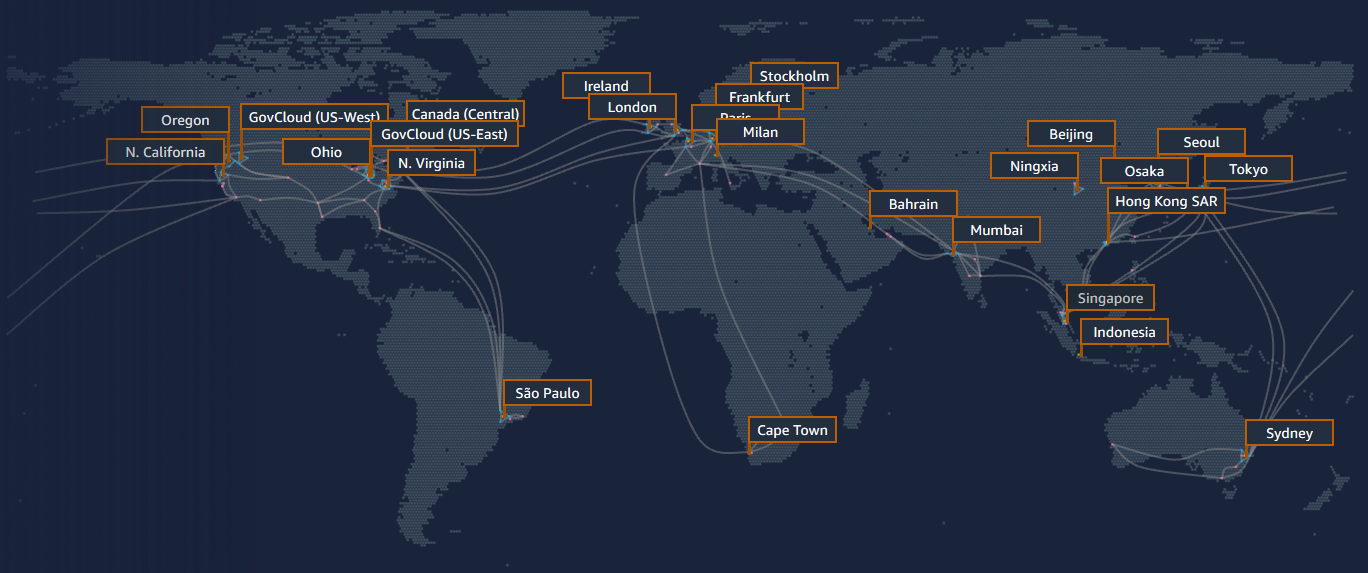
\includegraphics[width=\textwidth]{assets/aws_infrastructure.png}
  \caption{Regions of AWS}
  \label{aws_regions}
\end{figure}

\subsection{Existing Solutions}
\label{existing_solutions}
% Existing solutions and issues
  % Mainframes
    % inflexible
    % high maintenance
    % single point of failure
    % very expensive
    % more
  % "edge" / "gateway" nodes
    % essentially just small data centres
    % similar downsides
  % NetFPGA
    % doesn't solve problem
  % SDN
    % doesn't solve problem

  % Other drawbacks
    % security
    % scalability
    % Flexibility
    % performance

Some methods have been designed to reduce the time taken for data to travel between a user and a cloud server.
One of these methods is `edge' or `gateway' nodes.
Edge nodes are comparable to datacentres, with the key difference being that they are significantly smaller. They exist to hold content closer to users, so that not all content needs to be retrieved all the way from the data centre. Edge nodes are often used to host tools intend to manage the data centre, such as tools for customers to manage the data they have stored on a cloud computing platform.

While edge nodes do improve the service, they suffer from many of the same drawbacks as data centres do. In addition, the more edge nodes cloud computing platform creates, the more difficult it is for them to manage their hardware, as it becomes more spread out.

Before cloud computing became widely popular, it was necessary for users to host their own files. For those with large data requirements, it was not uncommon to use mainframe computers. These are large, high performance server computers, generally built and sold as a unit. Those using a mainframe would process all of their data on site. This would allow for data to be processed with an extremely low latency.

However, mainframe computers became unpopular for all the reasons cloud computing grew popular. Mainframe computers require significant on-site management. They require a high up-front cost, constant running costs in terms of power and cooling, are physically large and loud, and can be difficult to scale.

\subsection{Project Solution}
\label{project_solution}
% Why this, and why this is different?
  % Don't divert data from current path.
    % It's heading to data centre, so use that path.
  % choose appropriate device
    % ASIC vs FPGA vs CPU


The approach this project has taken to solving this problem has been comprised of two parts. Firstly, by not altering the path of the data, any data which would need to travel the full path would not be slowed. Secondly, choosing an appropriate device to perform the computation.

\subsubsection{Maintaining Data Path}

This approach lead to the idea of FPGA-based smart network switches. These switches could replace standard network switches, and would be able to perform small amounts of computation on data as it passed through these switches. If data was able to be fully processed by the switch, it would then be returned to the device, without ever needing to send it to the data centre. If the switch was unable to complete the computation within a set amount of time, it would release the data in its partially processed state along its original path, where it would then meet either further FPGA-based smart network switches, or its destination server. If it met further FPGA-based smart network switches prior to reaching its destination server, these could perform additional processing on the data, leading to a higher chance of completing the computation for a set of data.

\subsubsection{Choosing a Device for Computation}

The devices considered for use as computation devices in these smart switches were FPGAs, ASICs, and CPUS. Each of these have different advantages and disadvantages over one another. Three of the main areas of comparison were speed, flexibility, and cost.

The fastest of these three devices are ASICs. ASICs compute the algorithm they are designed for in hardware, and they are capable of doing so very efficiently.
Since FPGAs are designed to be more flexible than ASICs, ASICs can achieve greater speeds than FPGAs for the same algorithm.
CPUs are significantly slower than both ASICs and FPGAs, since they perform computation in software, rather than in hardware. In addition, unlike ASICs and FPGAs, CPUs are not standalone devices. They require additional hardware in order to function, including RAM, a motherboard, potentially storage, and often additional cooling. This would mean that any data the CPU would need to process would have to flow through an Ethernet interface which, for a high bandwidth Ethernet connection would likely need to be a NIC connected through a PCIe interface, then through the motherboard, then the RAM, then the CPU cache, then the CPU registers, before it could be processed. While there will also be more than one stage to process data using an FPGA or ASIC, this is far more complex with a CPU.

While ASICs are the best for speed, they are the worst for flexibility. ASICs are by definition application-specific, meaning that they are designed to perform one algorithm, and that is the only algorithm they are capable of performing. In order to achieve the flexibility required for this project, different ASICs would need to be designed for each algorithm required by a user, and the smart switches would then have to be physically swapped out to change the algorithm. This would also be inordinately expensive, and is unlikely to be manufacturable.
FPGAs are significantly more flexible than ASICs. They can be programmed using either HDLs such as \textit{Verilog} or \textit{VHDL}, or some high-level languages such as \textit{C} or \textit{C++} using sophisticated synthesis tools. In addition, FPGAs support advanced techniques such as `Partial Reconfiguration', which allows blocks of an FPGA to be declared as `reconfigurable', and these blocks can then be swapped out during runtime, without stopping the execution of the remainder of the program running on the FPGA.
CPUs are the most flexible of the devices, again due to their ability to run programs in software. This allows them to run programs using most modern programming languages, including 2019's most loved languages, \textit{Rust} and \textit{Python} \cite{stack_overflow_dev_survey_2019}.
However, as mentioned above, CPUs are not standalone devices. Their requirement for additional hardware restricts their flexibility, since it increases their physical size.

Finally, cost is the most difficult to compare devices, since there are many different parameters to take into account. The cheapest devices available are consumer CPUs, which can cost less than £100 for a low end desktop CPU \cite{scan_celeron_g4900} \cite{intel_celeron_g4900}, or over £2000 for a high end server CPU \cite{scan_xeon_gold_6132} \cite{intel_xeon_gold_6132}.
However, these are consumer prices, and assume the purchase of only one product.
However, even these prices cannot be considered entirely accurate, since they assume the purchase of only one device.
FPGAs and ASICs are more difficult to find accurate prices for, however a comparison of the two can be seen in figure \ref{fpga_asic_cost_tradeoff}. ASICs have a much higher initial cost, but a lower cost per unit compared to FPGAs.
However, FPGAs are a very active research area, and their cost per unit is slowly decreasing, causing the break even point shown in figure \ref{fpga_asic_cost_tradeoff} to slowly shift to the right, making FPGAs more favourable than ASICs.

FPGAs were chosen as the optimal computation device for this project. ASICs are insufficiently flexible, and even with their advantages in speed, they are subsequently not suitable for this task. CPUs, while more flexible than FPGAs, are significantly slower, and would be impractical to combine with a network switch. FPGAs are fast, flexible, and sufficiently small devices, and are the most suitable tool available.

\begin{figure}[ht!]
  \centering
  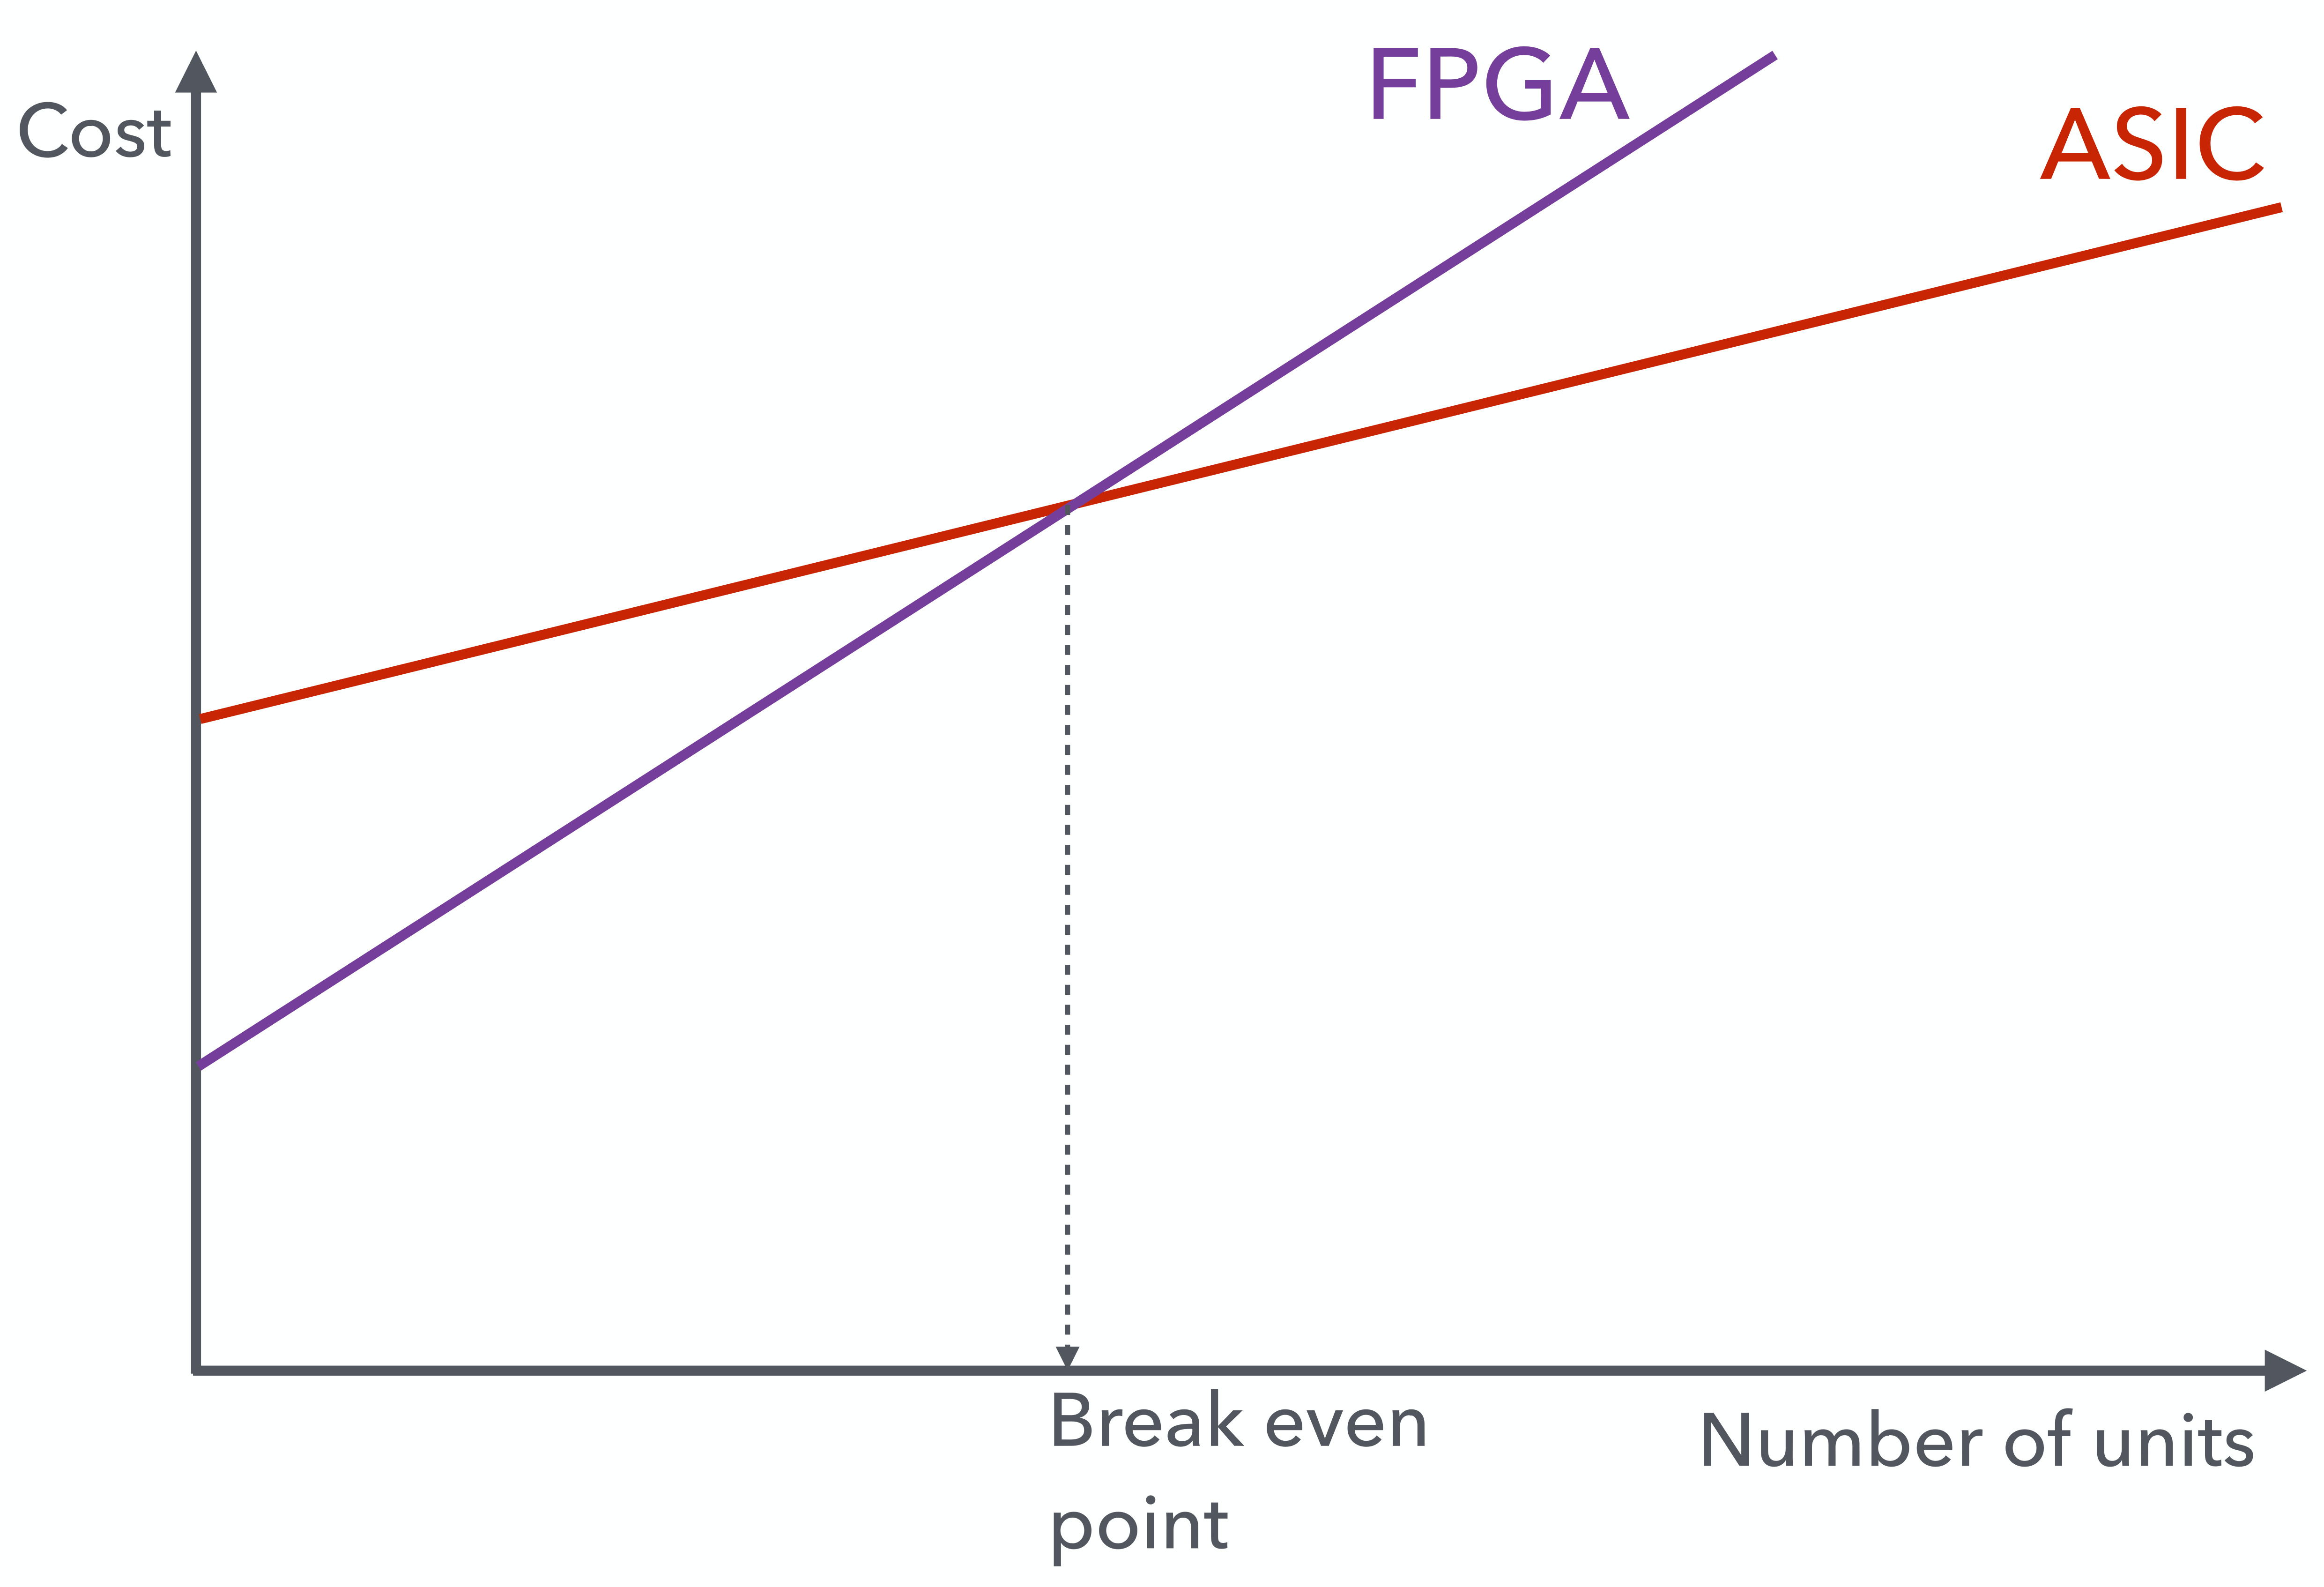
\includegraphics[width=\textwidth]{assets/fpga_asic_cost_tradeoff.png}
  \caption{Comparison of FPGA and ASIC cost \cite{es3b2}}
  \label{fpga_asic_cost_tradeoff}
\end{figure}


% Why FPGAs?
  % Custom compute architectures - very low latency
  % why not CPU? (bring data in through NIC -> mobo -> mem -> cache -> reg -> CPU -> back out)
    % FPGA just in and out
  % Partial reconfiguration


\section{Project Aims}
\label{project_aims}
% This is what we're aiming to do with the project.
% In our case, it's create this python script.
% It's not, it's the FPGA-based smart switches. The python script is simply the implemented aspect.

% So what we want to be doing is talking about the research.
%   Use words like investigate a lot.
%   Look at the aims of the other projects.

% It's also very important to talk about the reasoning behind all of the aims

% Create an application to model networks containing FPGA-based smart switches
% Allow users to test whether FPGA smart switches would be suitable in their network

% Something to do with implementing on NetFPGA?
% Something to do with SDN, control plane


% Coles:
%   Connect platforms
%   Connect people
%   use simple techniques
%   provide recommendations

%%% STRUCTURE %%%%

% Coles
  % Different subsections for each aim
  % 3 - 6 aims

% Dutton
  % no subsections
  % 1 overarching aim, 1-2 sub aims

% Thompson
  % Talk about how the aims changed after the project started
  % i.e. initially the aims were to build the hardware, but that changed to be more research focus


The main aim of this project is to research the complexities of creating an FPGA-based smart network switch. This is a notable change from the initial aims of the project, which were more focused on implementation rather than research. However, due to the agile nature of the project, discussed further in section \ref{project_management}, it was possible to make this change.
The initial implementation focused aims of the project were found to limit the project from exploring certain areas of research which proved both relevant and interesting. In addition, re-evaluating the feasibilty of the initial project aims after meeting certain external delays, even while using the risk mitigation strategies laid out in section \ref{risk_management}, indicated that that these updated project aims would be less susceptible to similar delays.

\subsection{Research FPGA-Based Smart Network Switch}
This is the primary aim of the project. These devices are currently entirely theoretical, and as a result more research than is feasible in this project will be required before these devices are close to being commercially available. As a result, the research into these devices, along with the complicatinos of their design and implementation is being prioritised over the actual implementation of one such device. This will allow for the project to investigate the theory of FPGA-based smart network switches in more depth.

\subsection{Model FPGA-Based Smart Network Switches}
A further aim of the project is to design and implement a model of the FPGA-based smart network switches in order to demonstrate their potential advantages over a standard connection to a server in a data centre. This should allow users to test whether FPGA-based smart network switches would be suitable in their network, and to design their network architecture accordingly if they are. 


\section{Project Stakeholders}
\label{project_stakeholders}
% Manufacturers of devices
  % FPGAs
    % Xilinx
    % Altera
  % Switches
    % HP
    % Cisco
    % Netgear
    % D-Link
% Users
  % Hospitals
  % Schools
  % Offices
  % Military
  % within datacentres - data going around centre
  % IoT
% Academia
  % Expanding research area?
  % NetFPGA community?
  % Mininet commuity?



\chapter{Research}
\label{research}
\section{Software-Defined Networking}
\label{software_defined_networking}
% reference mininet and P4
% control plane vs data plane
  % what are these
  % Why is it good to separate them?
  % what are the drawbacks of separating them?

% from progress report
The primary benefit of SDN is that it gives the programmer more direct and clear control over how routing decisions are made. SDN aims to separate the network control, known as the control plane, from the forwarding proces, known as the data plane \cite{software_defined_networking_survey}. The control plane makes decisions about packets which are either destined to or originally from the current host, while the data plane makes decisions about packets which are going through the host. The control plane also maintains the routing table, which is used by both planes to make routing decisions.


\section{Mininet}
\label{mininet}
% What is mininet
% The python API
% It is python based, which is good and bad
% It brings in a dependency chain
% It is flexible in some ways (e.g. the topology)
% It is restrictive in others

% SDN with OpenFlow

Mininet is an open-source network emulator written primarily in \textit{Python} \cite{mininet}. It is intended for use in creating virtual networks, and can be used to design custom network topologies and test different performance characteristics of these networks.
\textit{Wireshark}, the popular network protocol analyser \cite{wireshark}, can be integrated into mininet, allowing network packets sent within a virtual mininet environment to be easily captured and analysed.
Mininet also provides a \textit{Python} API, allowing it to be easily integrated within other applications, and for complex topologies to be constructed using \textit{Python}.
It is very lightweight, with the total size of the source code being less than 1MB.
Using Mininet will naturally introduce a dependency chain. However, this is the case with most open-source software, and due to its lightweight nature there are a relatively small number of dependencies.
Mininet uses CI testing through \textit{Travis CI} \cite{travis_ci}, which will run all unit and integration tests upon every commit to the Mininet \textit{GitHub} repository \cite{github}. These tests can be checked to improve the reliability of Mininet.

Currently, the latest stable release of Mininet is version 2.2.2, which was released on 21 March 2017. This is supported on Ubuntu 14.04 LTS, and is not supported on newer versions of Ubuntu (or other distributions) due to an incompatibility between this version of Mininet and the Linux 3.16 (or newer) kernel. As a result, software which uses Mininet 2.2.2 will also be unsupported on versions of Ubuntu newer than 14.04 LTS.

The fifth release candidate for Mininet 2.3.0 was released on 14 March 2019, and it is expected that when Mininet 2.3.0 is released, it will be supported on Ubuntu 18.04 LTS.


\section{P4}
\label{p4}
% When was it started
% Is this good or bad
% What has it been used for
% advantages and drawbacks of it
% Isn't it C based or something?


\textit{P4} is a language used in SDN for programming the data plane of network devices \cite{P4}. The specification for $P4_{14}$ (the first version of P4) was released in September 2014. This went through a few minor revisions before the specification for $P4_{16}$ (the current version) was released. \textit{P4} is a language which could be used on a FPGA-based smart network switch in order to control how packets are processed through the switch, however is not used in the implementation aspect of this project.

% From progress report
% P4 is a language for programming the data plane of network devices \cite{P4}. The specification for $P4_{14}$ (the first version of P4) was released in September 2014. This went through a few minor revisions before the specification for $P4_{16}$ (the current version) was released. This project will use $P4_{16}$.


\section{NetFPGA}
\label{netfpga}
% different platforms
  % 1G
  % 10G
  % SUME
  % CIVIL
  % pros and cons
% Why NetFPGA
% What does NetFPGA provide
% standalone and integrated



\chapter{Requirements}
\label{requirements}
\section{Initial Requirements}
\label{initial_requirements}
% Get these from specification and progress report
% Add some commentary about how they are outdated because
  % they reflect the system you were building at the start of the project
  % You're agile, so it changed
  % the new system is better and more feasible
  % reference the new ones
  % reference the spec
% have subsections for func and non func


\section{Functional Requirements}
\label{functional_requirements}
% base off spec, but adapt to new system
% have a brief description of func reqs (what they are)

The functional requirements describe the technical capabilities of the implemented aspect of the project.
They detail how the system should react in certain scenarios, and state what services the system should be able to provide.
The can also state limitations in the scope of the system, i.e. routes of development that are not intended to be implemented \cite{software_engineering_req_analysis}.

\begin{enumerate}[label=\textbf{F\arabic*:}]
  \item The system \textbf{must} allow the modelling of a network with at least three switches and four hosts, arranged in a tree topology as shown in figure \ref{minimum_tree}.
  \item The system \textbf{must} allow switches and hosts to be configured in a tree topology.
  \item The system \textbf{must} allow users to specify the spread of the network when using a tree topology (i.e. how many children a switch node will have).
  \item The system \textbf{must} allow users to specify the number of levels in the network when using a tree topology.
  \item The system \textbf{must} allow users to specify which level in the network should be modelled as FPGA-based smart network switches.
  \item The system \textbf{must} allow users to run a test to ensure there is an active connection between all hosts.
  \item The system \textbf{must} allow users to run a test to display the bandwidth of the system.
  \item The system \textbf{must} allow users to run a test to display the delay between the leaf nodes and the root when using a tree topology.
  \item The system \textbf{should} allow users to specify the bandwidth of all links in the network.
  \item The system \textbf{should} allow users to specify the delay of all links in the network.
  \item The system \textbf{should} allow users to specify the chance of packet loss for all links in the network.
  \item The system \textbf{should} allow switches and hosts to be configured in a vertical linear topology.
  \item The system \textbf{should} employ multiple levels of logging.
  \item The system \textbf{should} conform to \textit{Python}'s PEP8 code standard \cite{python_pep8}.
  \item The system \textbf{should} be made open-source.
  \item The system \textbf{could} allow users to configure the system to use a Poisson distribution for link delays.
  \item The system \textbf{could} allow users to configure the bandwidth of FPGA-based smart network switch nodes.
  \item The system \textbf{could} allow users to configure the delay of FPGA-based smart network switch nodes.
  \item The system \textbf{could} allow users to configure the chance of packet loss of FPGA-based smart network switch nodes.
  \item The system \textbf{could} allow users to display all node connections before running tests.
  \item The system \textbf{won't} be configured for IPv6 connections.
\end{enumerate}


\begin{figure}[t]
  \centering
  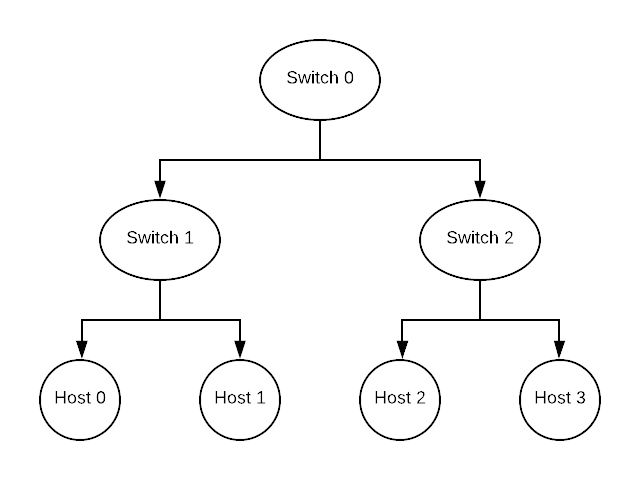
\includegraphics[width=\textwidth]{assets/minimum_tree.png}
  \caption{The Required Minimum Tree Topology}
  \label{minimum_tree}
\end{figure}

% \begin{enumerate}[label=\textbf{F\arabic*:}]
%   \item The system \textbf{must} be able to analyse packets at layer 2 of the OSI network model
%   \item The system \textbf{must} be able to send packets to the correct port based on MAC addresses
%   \item The system \textbf{must} be able to store MAC address tables
%   \item The system \textbf{must} be able to dynamically update MAC address tables
%   \item The average latency of the system \textbf{must} be measured
%   \item The throughput of the system \textbf{must} be measured
%   \item The system \textbf{should} be able to analyse packets at layer 3 of the OSI network model
%   \item The system \textbf{could} be able to analyse packets at layer 7 of the OSI network model
%   \item The system \textbf{could} be able to detect basic network attacks (such as TCP SYN Flooding \cite{rfc4987})
%   \item The system \textbf{could} implement features of a basic firewall (such as packet filtering \cite{rfc2979})
% \end{enumerate}


\section{Non-Functional Requirements}
\label{non_functional_requirements}
% base off spec, but adapt to new system
% have a brief description of non func reqs (what they are)

These requirements describe the general operation of the system produced, as well as how the project should be developed. They often apply to the system as a whole rather than targeting individual components, and they can include any legislative constraints on the system.

 \cite{software_engineering_req_analysis}.

 \begin{enumerate}[label=\textbf{NF\arabic*:}]
     \item The system \textbf{should} be scalable
     \item The system \textbf{should} be efficient
     \item All code for the system \textbf{should} be well-documented and maintainable
 \end{enumerate}

 % \begin{enumerate}[label=\textbf{NF\arabic*:}]
 %   \item The system \textbf{should} be scalable
 %   \item The system \textbf{should} be efficient
 %   \item All code for the system \textbf{should} be well-documented and maintainable
 % \end{enumerate}


\section{Project Constraints}
\label{project_constraints}
% Python is slow
% People have slow computers
% Mininet only runs on ubuntu 16
% Python 2
% Switches 1U rack (usually)
% switches standard rack depth (but normally half or less)
% Python minimum operating reqs
% mininet minimum operating reqs
% Deadlines etc



\chapter{Ethical, Social, Legal, and Professional Issues}
\label{issues}
\section{Ethical Issues}
\label{ethical_issues}
% Privacy
% GDPR
% anonymous results?
% storing personal information

The primary ethical for this project was privacy. While no user data is directly required for this project, a wide variety of data would naturally pass through a complete FPGA-based smart network switch.
As a result, when designing these devices, or even just considering the foundation for them, it is important to ensure that they are secure, and would be resistant to malicious attempts to read data passing through the switches.

This can link to the physical media discussed in section \ref{physical_media_research}. Fibre optic cable is significantly more secure than UTP copper cable, which is susceptible to `tapping', where an additional cable can be attached to the original copper cable, and this can be used to read the data flowing through it. This technique is extremely difficult with fibre optic cable, since attempts to do so will almost always break the cable.
This ethical issue should influence the design of the FPGA-based smart network switches, and the types of physical media with which they are compatible.


\section{Social Issues}
\label{social_issues}
% Don't check sexual / religious / polictical status to avoid victimising someone?
% Or race / disability
% don't dsicriminate
% How does app impact society?
%
% languages
% UI?


\section{Legal Issues}
\label{legal_issues}
% Use of third party tools
% Licensing
% aim to use open source
% Data Protection Act 1998
% GDPR
%
% how was data obtained?
% "I abided by terms of use"
% If you agreed to any terms and conditions, what do they say? are there consequences?
%
% liability:
%   could a user injure themselves while useing system (obvs not)
%   could a user damage their network using system?
% Copyright?
% patenting
%
% APIs
% watermarking
% what license are you providing the software to be used?
% software license agreement?

When using third tools, it is important to ensure that they are being used in accordance with the licence with which they are provided.
Much open-source software is provided with either the \textit{Apache License 2.0} \cite{apache_2_0}, the \textit{GNU General Public License v3.0} \cite{gnu_gpl_3}, or other similar licences allowing conditional free use of the software.
As a result, this project will aim to use open-source tools where they are available to avoid issues with copyright.

Two Regulations this project will be additionally careful not to contravene are the \textit{General Data Protection Regulation 2016} \cite{eu_2016_679} and the \textit{Data Protection Act 2018} \cite{uk_dpa_2018}. These Statutes involve the storage, collection, and processing of data, and relate to the issues descibed in sections \ref{ethical_issues} and \ref{social_issues}.

Wherever secondary data (i.e. data not directly collected by the developer) has been used, any conditions to the use of this data must be considered. Should any terms of use relating to the data be accepted, these must be adhered to, and the primary stakeholders outlined in section \ref{primary_stakeholders} should be aware of any consequences that could occur from breaching these terms of use.


\section{Professional Issues}
\label{professional_issues}
% "As a member of the BCS"
% Follow BCS code of conduct / code of practice?
% say something about how I aim to follow BCS code of conduct anyway
% Follow industry standars
%
% user's sense of security maintaines so user feels they can trust the app
%
% describe in what ways you're following BCS

Since the developer is a member of the BCS, following the BCS Code of Conduct \cite{bcs_code_of_conduct} is a general professional aim, not limited to the scope of this project. The BCS Code of Conduct comprises four key principles:
\begin{enumerate}
  \item You make IT for everyone
  \item Show what you know, learn what you don't
  \item Respect the organisation or individual you work for
  \item Keep IT real. Keep IT professional. Pass IT on.
\end{enumerate}

These principles have been consciously followed throughout this project. By making the implemented aspect of the project open-source, the first principle is being followed. The IT application created as a result of this project is being made available for everyone. This project has involved a great deal of learning for the developer in order to gain the necessary skills to research and develop the project. In addition, the background knowledge discussed in section \ref{background_knowledge} was used as a basis for the project. This demonstrates the second key principle. The third key principle has been taken into account whenever in contact with members of the University of Warwick. Finally, this project represents a key area of interest for the developer who has been motivated to develop and share the knowledge acquired over the course of the project, exemplifying the fourth key principle.



\chapter{Design}
\label{design}
% Mininet
% virtual Network
% custom toppologies
% modelling fgpa smart switches
% distinction between FPGA-based smart network switches  and regular

% initially, just do regular

% iterative design, so system should always be working, and one feature was added at a time, along with tests

% key features were...

% talk about pylint, integrated with pycharm

% travis?

% poisson feature

% git submodules
  % talk about how you thought about including the code from mininet, and keeping it up to date
  % YOU HAVEN'T MENTIONED SUBMODULES ANYWHERE ELSE!
  % talk about how mininet is developed in git on github

  % the same approach could be used for other shit in future

% I thought about documentation,
  % Readme was sufficient

% click vs argparse

% logging

After completing the initial research and constructing the requirements for the system, the development of the system began.
Due to the agile methodology of the project, development was conducted incrementally, with each feature being developed sequentially along with its associated tests and documentation.
This provides the advantage of the system being functional throughout the process of development, and allows for flexibility of how the development process occurs.
However, this makes it challenging to separate the design of the system from its implementation, since these both occurred throughout development for each individual feature.
Regardless, to provide a clear overview of the development process they have been separated for the purpose of the report, and the design of the system is discussed in this section.

\section{Tool Selection}
\label{tool_selection}

\subsection{Network Simulation}

Since the primary purpose of the system is to model networks, an application needed to be sourced to simulate these networks.
While this application could have been implemented from scratch as part of the project, which would have thereby have eliminated any associated licencing or dependency issues, this was deemed to be an inefficient use of time since this software already exists, and would be complex to implement.
\textit{Mininet} was chosen for this purpose since it is open-source, has a wide array of features, and integrates well with SDN using its custom version of \textit{OpenFlow} \cite{mininet_openflow}.
\textit{OpenFlow} is a ``flow-based switch specification designed to enable researchers to run experiments in live networks''.
Similar to \textit{P4}, \textit{OpenFlow} can be used to manually control the data flowing through a network switch, and \textit{Mininet} supports this protocol directly.

\subsection{Programming Language}

\textit{Python} \cite{python} was chosen as the primary programming language for the project.
\textit{Mininet}'s API is written in \textit{Python}, and \textit{Python} includes many tools which can be used to ease the development of an application.
\textit{Python}'s style guide, \textit{PEP 8} \cite{python_pep8}, can be used to ensure an application is written according to the standards used in industry, and tools such as \textit{Pylint} can notify the developer if any code written does not meet this.

\section{Open-Source}
\label{open_source}

The system being made open-source contributed to the development approach.
\textit{GitHub} \cite{github} was used to make the code open source, and \textit{git} \cite{git} is the version control system used by \textit{GitHub}.
\textit{Git} tracks changes in the form of `commits', which constitute a defined set of changes made to the code, accompanied by a short message summarising the changes.
Commits are a core concept of \textit{git}, however \textit{git} contains many additional features pertaining to managing the source for a project.
Many of these features are complex, and as a result care needs to be taken when using \textit{git} for an open-source project that it is used in an appropriate way.
Each commit should be used for exactly one step in development, where these steps are suitable sized such that each step is as small as possible, while ensuring that the system functionality is maintained with every commit.
In other words, no commit should decrease the functionality of the system, unless that is the intended purpose of the commit.

Another core concept of \textit{git} is `branches'.
Each branch contains a replica of the project source, from the point in time when the branch was created.
Each branch is totally independent of every other branch, and there is no limit to the number of branches which can be created.
This means that two different features can be developed simultaneously without impacting one other, by developing each one on its own branch.
Branches are also able to be `merged' into one another, appending all of the commits from one branch onto the branch it is being merged into.
This feature was used heavily throughout the development of the project, with every feature being developed in its own branch before being merged into the primary branch of the project, known as the `master' branch.

\section{Dependencies}

Since the project included dependencies, a reliable way of delivering the system with these dependencies was required.
While the source code for all dependencies could be manually copied into the repository for the system, this would then require manually copying the code for every dependency whenever updates are released, and would also increase the size of the system.
For all \textit{Python} libraries used (which would normally be installed using \textit{Python}'s \textit{Pip} package manager), the \textit{Python setuptools} \cite{python_setuptools} library was used.
This is installed by default with every installation of \textit{Python}, and allows for \textit{Python} dependencies to be specified in a \textit{Python} file which defines setup characteristics of the application.
Whenever an application which uses \textit{setuptools}, such as this system, is installed using \textit{Pip}, \textit{Pip} will then check the \textit{setuptools} file for the list of dependencies, and also install these.

The only dependency used by the project which could not be included in this way was \textit{Mininet}.
Since \textit{Mininet} is open-source, and its code is available in a \textit{git} repository on \textit{GitHub}, it was decided to use \textit{git submodules} in order to register \textit{Mininet} as a project dependency.
\textit{Git submodules} are a feature of a \textit{git} which allows a \textit{git} repository to declare further \textit{git} repositories that it uses.
These additional repositories will then be downloaded with the source code for the main system whenever it is downloaded using the `--recursive' flag.
\textit{Git submodules} can also be attached to a particular commit of a repository, and this has been used to attach the submodule of \textit{Mininet} to its version 2.2.2 release.
When a new stable version of \textit{Mininet} is released, this can be tested, and then updated simply be changing the version number in the \textit{git submodules} configuration file.


\chapter{Implementation}
\label{implementation}
% NOTES FROM DESIGN %

% Mininet
% virtual Network
% custom toppologies
% modelling fgpa smart switches
% distinction between FPGA-based smart network switches  and regular

% initially, just do regular

% iterative design, so system should always be working, and one feature was added at a time, along with tests

% key features were...

% talk about pylint, integrated with pycharm

% travis?

% poisson feature

% git submodules
  % talk about how you thought about including the code from mininet, and keeping it up to date
  % YOU HAVEN'T MENTIONED SUBMODULES ANYWHERE ELSE!
  % talk about how mininet is developed in git on github

  % the same approach could be used for other shit in future

% I thought about documentation,
  % Readme was sufficient

% click vs argparse

% logging

% NOTES FROM DESIGN %
% ----------------------------

% Initially, no options.
%   Based off Mininet example.
%   Simple Mininet tree Topology
%   Essentially a Mininet wrapper
%   git submodule
%   .gitignore
%
%
% Then added structure
%   Readme?
%   argument parsing
%     argparse vs click
%   travis structure
%
%
% logging
%   json config
%
%
% performance tests
%   custom cloud test
%   mininet tests
%
%
% further options
%   spread
%   depth
%   bandwidth
%   delay
%   loss
%   fpga
%   fpga-bandwidth
%   fpga-delay
%   fpga-loss
%   ping-all
%   iperf
%   cloud-fpga
%   dump-node-connections
%   poisson
%   log
%
% user testing?

\section{Initial System}
\label{initial_system}
% Initially, no options.
%   Based off Mininet example.
%   Simple Mininet tree Topology
%   Essentially a Mininet wrapper
%   git submodule
%   .gitignore
The system was initially implemented as a wrapper for the \textit{Mininet} API.
This would utilise the relevant features of the API, while restricting access to those which were not relevant to the system.
This involved declaring \textit{Mininet} as a \textit{git submodule} of the system, as discussed in section \ref{dependencies}.
The implemented features of the \textit{Mininet} API were a simple tree topology, and a network test built into the API which would confirm that all hosts in the topology could communicate with one another.
Once these had been implemented, running the system would:

\begin{enumerate}
  \item Initialise the network
  \item Create the required switches
  \item Create the required hosts
  \item Create the required links between switches and other switches, and between switches and hosts
  \item Run the network test and display the results
  \item Break down the network.
\end{enumerate}

\section{System Structure}
\label{system_structure}
% Then added structure
%   Readme?
%   argument parsing
%     argparse vs click
%   travis structure
%

With the core functionality in place, structure could now be added to the system to allow additional features to be added in a sustainable and efficient way.
% Write some more here

\subsection{User Customisation}
\label{user_customisation}
For command line applications such as this one, customisation is commonly performed through either configuration files, or through arguments specified at the command line.
For this system, command line arguments were deemed more appropriate, since they allow for a simpler user experience, while still providing a high level of flexibility.
The \textit{Python} library \textit{Click} \cite{python_click} was used to implement these arguments.
\textit{Click} was chosen since it allows for a large amount of customisation of the system's arguments.
By default, \textit{Click} configures the `--help' flag, which will print out a formatted list of all available flags and arguments for the system, along with the type of data they expect and any explanatory messages associated with each flag or argument.
For each flag or argument, the type can be configured, as can the explanatory message, and the name of the flag or argument.
A default value can also be set, and custom restrictions can be placed on the type of data accepted by each flag or argument.

\subsection{Documentation}
\label{documentation}
Suitable documentation was required to ensure the usability of the system.
A separate user guide was considered. However, it was concluded that this was unnecessary, due to the straightforward nature of the command line interface.
Instead, a `Readme' file was written in \textit{Markdown} \cite{markdown} and added to the \textit{GitHub} repository for the system where it would be formatted and clearly displayed.
% More

\subsection{Testing Structure}
\label{testing_structure}
% \textit{Travis CI} \cite{travis_ci} was used to conduct many of the tests in the system.
\textit{Travis CI} \cite{travis_ci} is a web-based CI platform designed for running automated tests, and this was used to conduct many of the tests in the system.
The testing process itself is discussed in detail in section \ref{testing}.
However, prior to tests being written, \textit{Travis CI} needed to be configured to automatically run tests on changes it detected in \textit{GitHub}.
To do this, a \textit{YAML} configuration file for \textit{Travis CI} was added to the code.
A directory was also created for tests to be added to.

\section{Feature Implementation}
\label{features}
Features could now be implemented on the system.
The development approach up to this point would allow for each feature to be added into the system without needing to be concerned with anything other than that feature.
Features were added sequentially, along with their required \textit{Click} configuration, their tests, and their documentation.

\subsection{Logging}
\label{logging}
The first feature to be added was standardised logging.
This was done using \textit{Python}'s \textit{logging} \cite{python_logging} package, which is designed for this purpose and is highly customisable in how its logs are recorded.
The logging package uses concepts of `loggers', `handlers', and `formatters'.
A logger receives log messages from a system, and dispatches these to a set of defined handlers.
The handlers will then process the log messages, according to the formatters they are linked to.
A formatter simply defines a format of a log message.
For this system, one standard formatter was used, which was defined as \codeword{%(asctime)s - %(name)s - %(levelname)s - %(message)s}.
This formatter would print the current date and time, followed by the name of the logger, followed by the log level used for the message, followed by the actual log level.

The logging package supports six log levels which are each associated with an integer value.
These are shown in table \ref{log_levels}.
Whenever a message is logged by the system, it is logged using one of these levels.
A user can specify the mininum log level to be displayed, and then all log messages of this level or higher will be displayed.
If no level is specified, the system defaults to INFO.

\begin{table}[t]
  \caption{Log Levels for \textit{Python} \textit{Logging} Package}
  \begin{center}
    \begin{tabularx}{\textwidth}{|Y"Y|} \hline
      \textbf{Log Level} & \textbf{Numeric Value} \\ \thickhline
      CRITICAL & 50 \\ \hline
      ERROR & 40 \\ \hline
      WARNING & 30 \\ \hline
      INFO & 20 \\ \hline
      DEBUG & 10 \\ \hline
      % NOTSET & 0 \\ \hline
    \end{tabularx}
  \end{center}
  \label{log_levels}
\end{table}

The majority of the configuration for the logging package was placed in a \textit{JSON} file.
Three log handlers were specified in this file.
These handlers logged all messages with a log level greater or equal to the system's minimum log level.
Each handler logged the messages to a different location, and had a different hard minimum log level of messages it would record, shown in table \ref{log_handlers}.
The log files used were automatically rotated by the \textit{logging} package, such that when the log files reached 10MB in size, the data would be moved to an old file, and a new file would be created.
A maximum of 20 backup log files would be kept for each of the two handlers which logged data to files.

\begin{table}[t]
  \caption{Log Handlers Used}
  \begin{center}
    \begin{tabularx}{\textwidth}{|Y"Y|} \hline
      \textbf{Log Target} & \textbf{Hard Minimum Log Level} \\ \thickhline
      Console & DEBUG \\ \hline
      Log file `fpga\_switch\_model.info.log' & INFO \\ \hline
      Log file `fpga\_switch\_model.error.log' & ERROR \\ \hline
    \end{tabularx}
  \end{center}
  \label{log_handlers}
\end{table}

%   log
%   dump-node-connections

\subsection{Performance Tests}
\label{performance_tests}
% performance tests
%   custom cloud test
  %   cloud-fpga
%   mininet tests
  %   ping-all
  %   iperf

Functions were implemented to allow users to measure the performance of the virtual networks created by the system.
The initial system described in section \ref{initial_system} included a simple test to confirm all hosts could communicate with one another.
This test was based on the `ping' network utility, which sends an ICMP packet from one host to another, and measures the round trip time for the packet.
The test used in the initial system, known as a `ping-all' test, iterates through every host in the virtual network pinging every other host, and confirms that a response is received to every ping.
This test was configured so that it would only be executed if the system was started with the `-p' or `--ping-all' flags.

\textit{Mininet} also includes a test to measure the bandwidth of the virtual network, based on the \textit{iperf} \cite{iperf} tool.
This test was added to the system, and was configured so that it would only be executed if the system was started with the `-i' or `--iperf' flags.

At this stage of implementation, the topology of the virtual network created by the system was limited to a tree topology which could not be modified.
However, by the end of the implementation stage, the depth and spread of the tree topology would be customisable, and the user would be able to specify a level of the tree to be modelled as FPGA-based smart network switches.
With this in mind, an additional performance test was written which would measure the round trip time between either the base and the root of the tree, or between the base and the FPGA-based smart network switch layer of the tree.
The purpose of this was to measure the time it would take a packet to be processed in the virtual network, if the root of the tree was thought of as `the cloud'.
This test was conducted by sending 10 packets using the ping network utility, and reading the utility's output.
This consisted of the minimum round trip time, average round trip time, maximum round trip time, and the standard deviation.
The test was configured so that it would be executed by default, although it could be disabled by setting the `-c' or `--cloud-fpga' flags to `False'.

\subsection{Network Topology Customisation}
\label{network_topology_customisation}
% further options
%   spread
%   depth
Two options were added to customise the topology of the virtual network.
The topology was still restricted to a tree, but the spread of the tree could be specified by the user with the `-s' or `--spread' flags, and the depth of the tree could be specified by the user with the `-d' or `--depth' flags.
If the spread was not specified by the user, it would default to two.
This value was chosen since this was the minimum spread which would still result in a tree topology.
A spread of one would result in a series of switches with a single host connected at the end.
If the depth was not specified by the user, it would default to four.
This value was chosen since this was the minimum depth which would allow a root node, a layer of FPGA-based smart network switches, a layer of standard switches, and a layer of hosts.

\subsection{Network Performance Customisation}
\label{network_performance_customisation}
%   bandwidth
%   delay
%   loss

%   poisson
Customisation options were then added to limit the performance of the virtual network, in order to bring the model closer to a real network.
One option which was added was to limit the bandwidth of the virtual network.
This limit would be applied to all of the links in the network, and could be specified using the `-b' or `--bandwidth' flags.
If this option was not specified, a limit of 10Mbps would be applied.
Another option applied a delay on all links in the network, and could be specified using the `-e' or `--delay' flags.
If this option was not specified, a delay of 1ms would be applied.
A futher option caused a chance for packets to be lost when passing through a link, and could be specified using the `-l' or `--loss' flags.
If this option was not specified, no chance of loss would be applied.

An option was also added to configure the network delay to be selected from a Poisson distribution for which the average is the current network delay.
This was designed to add an element of randomness to the system, again to bring this closer to a real network.
The `--poisson' flag could be used with the system to enable the use of a Poisson distribution for the link delay.

\subsection{FPGA-Based Smart Network Switch Customisations}
\label{FPGA_Based_Smart_Network_Switch_Customisations}

This set of options introduced FPGA-based smart network switches to the system.
With the `-f' or `--fpga' flags, a level of the tree topology could be specified to be modelled as FPGA-based smart network switches instead of regular switches.
These switches were implemented as regular switches linked to a host, where the link between them had double the possibility for packet loss compared to that of standard links, a bandwidth of 504Mbps, and latency twice that of standard links.
These hosts were treated as the FPGAs in the switches, and were used to respond to any pings directed to the switch, such as those used in the cloud-fpga test discussed in section \ref{performance_tests}.
The reason for this increased possibility for packet loss was that it was seen as more likely for packets to be lost inside an FPGA-based smart network switch compared to travelling along a wire, or when travelling through a standard switch.
The default bandwidth was set to 504Mbps since this is the maximum bandwidth of the PCIe interface, and it is assumed that an implemented FPGA-based smart network switch will incorporate the FPGA using an interface at least this fast.
The latency was increased to account for the time it would take to perform the computation on the packets in the switch before they are returned.

All of the performance characteristics described above can be customised using options added to the system.
The `--fpga-bandwidth' flag can be used to specify the bandwidth of the FPGA-based smart network switch links, the `--fpga-delay' flag can be used to specify their latency, and the `--fpga-loss' flag can be used to specify the probability of packet loss.


%   fpga
%   fpga-bandwidth
%   fpga-delay
%   fpga-loss

% \section{response to user testing?}


\chapter{Testing}
\label{testing}
% Travis
% Unit tests
% Integration tests
% system testing
% user testing
%   Show to isabelle, ask her what she thinks
%
% can be installed from source on clean install
% deploy to docker hub, testing there?
% deploy to pip, testing there?
%

Comprehensive tests were necessary in order to ensure that the implemented system functioned as intended.
The testing for this system was separated into unit, integration, system, environment, and user testing, as discussed further in the sections below.

As mentioned in section \ref{testing_structure}, \textit{Travis CI} \cite{travis_ci} is a web-based CI platform designed for running automated tests.
It was used for many of the tests in this project due to its clear interface, and easy integration with \textit{GitHub} repositories.
Whenever code was uploaded to \textit{GitHub}, \textit{Travis CI} would automatically run all configured tests on the code, and would notify the developer by email if any tests failed.
The testing environment used by \textit{Travis CI} can be easily configured using a single \textit{YAML} \cite{yaml} file located in the \textit{GitHub} repository for the project.



\section{Unit Testing}
\label{unit_testing}
Unit testing was conducted to ensure that each individual component of the system functioned as intended.
Tests were written for function in the code using a variety of different inputs, and the output of these tests was compared with the expected output.
The \textit{Python} library \textit{unittest} \cite{python_unittests} was used to write these tests, as it is designed for this purpose, and integrates easily with both the existing system and \textit{Travis CI}.
The results of the unit tests can be seen in a simplifed format in table \ref{unit_test_results}.

\begin{table}[t]
  \caption{Results of Unit Tests}
  \begin{center}
    \begin{tabularx}{\textwidth}{|Y|c|} \hline
      % \textbf{Unit Test} & \makecell{\textbf{Linked \\ Requirement(s)}} & \textbf{Success / Failure} \\ \thickhline
      \textbf{Unit Test} & \textbf{Success / Failure} \\ \thickhline
      Test \textit{halve\_delay} function & \textcolor{green}{SUCCESS} \\ \hline
      Test \textit{get\_poisson\_delay} function & \textcolor{green}{SUCCESS} \\ \hline
      Test \textit{test\_cloud\_fpga} function & \textcolor{green}{SUCCESS} \\ \hline
      Test \textit{TreeTopoGeneric} class & \textcolor{green}{SUCCESS} \\ \hline
      % 0 & 0 & 0 & 0 (A) \\ \hline
    \end{tabularx}
  \end{center}
  \label{unit_test_results}
\end{table}

\section{Integration Testing}
\label{integration_testing}
Integration testing was conducted to ensure the individual components of the system interacted with each other as intended.
Tests were written for different combinations of functions which were used together in the system using a variety of different inputs, and the output of these tests was compared with the expected output.
As with the unit tests discussed in section \ref{unit_testing}, the \textit{Python} library \textit{unittest} was used to write these tests.
The results of the integration tests can be seen in a simplifed format in table \ref{integration_test_results}.

\begin{table}[t]
  \caption{Results of Integration Tests}
  \begin{center}
    \begin{tabularx}{\textwidth}{|Y|c|} \hline
      % \textbf{Integration Test} & \makecell{\textbf{Linked \\ Requirement(s)}} & \textbf{Success / Failure} \\ \thickhline
      \textbf{Integration Test} & \textbf{Success / Failure} \\ \thickhline
      Test \textit{TreeTopoGeneric} class with \textit{get\_poisson\_delay} function class & \textcolor{green}{SUCCESS} \\ \hline
      Test \textit{TreeTopoGeneric} class with \textit{get\_poisson\_delay} function class & \textcolor{green}{SUCCESS} \\ \hline
      Test \textit{TreeTopoGeneric} class with \textit{halve\_delay} function & \textcolor{green}{SUCCESS} \\ \hline
      Test \textit{TreeTopoGeneric} class with \textit{test\_cloud\_fpga} function & \textcolor{green}{SUCCESS} \\ \hline
      Test \textit{TreeTopoGeneric} class with \textit{get\_poisson\_delay} function class and \textit{halve\_delay} functions & \textcolor{green}{SUCCESS} \\ \hline
      Test \textit{TreeTopoGeneric} class with \textit{test\_cloud\_fpga} and \textit{halve\_delay} functions & \textcolor{green}{SUCCESS} \\ \hline
      Test \textit{TreeTopoGeneric} class with \textit{test\_cloud\_fpga}, \textit{get\_poisson\_delay} and \textit{halve\_delay} functions & \textcolor{green}{SUCCESS} \\ \hline


      % 0 & 0 & 0 & 0 (A) \\ \hline
    \end{tabularx}
  \end{center}
  \label{integration_test_results}
\end{table}

\section{System Testing}
\label{system_testing}
System testing was conducted to ensure the system as a whole performed as intended.
The entire system was tested using different inputs for the available configuration options, and the output of the system was compared with the expected output.
The results of the system tests can be seen in table \ref{integration_test_results}.


\begin{table}[t]
  \caption{Results of System Tests}
  \begin{center}
    \begin{tabularx}{\textwidth}{|Y|c|c|} \hline
      % \textbf{System Test} & \makecell{\textbf{Linked \\ Requirement(s)}} & \textbf{Success / Failure} \\ \thickhline
      \textbf{System Test} & \textbf{Linked Requirement(s)} & \textbf{Success / Failure} \\ \thickhline
        Can the system function using a tree topology with a spread of two and a depth of four, with a total of 8 hosts? & F1, F2 & \textcolor{green}{SUCCESS} \\ \hline
        Can the system function using a tree topology with a spread of three and a depth of 8, with a total of 2187 hosts? & F1, F2, F3, F4 & \textcolor{green}{SUCCESS} \\ \hline
        Can the system report the bandwidth in the network? & F7 & \textcolor{green}{SUCCESS} \\ \hline
        Can the bandwidth in the network be configured correctly? & F9 & \textcolor{green}{SUCCESS} \\ \hline
        Can the link delay in the network be configured correctly? & F10 & \textcolor{green}{SUCCESS} \\ \hline
        Can the probability of packet loss in the network be configured correctly? & F11 & \textcolor{green}{SUCCESS} \\ \hline
        Can the link delay in the network be configured using a Poisson distribution correctly? & F16 & \textcolor{green}{SUCCESS} \\ \hline
        Can all node connections be correctly displayed? & F20 & \textcolor{green}{SUCCESS} \\ \hline
        Can the user specify the level of logging employed by the system? & F13 & \textcolor{green}{SUCCESS} \\ \hline

      % 0 & 0 & 0 & 0 (A) \\ \hline
    \end{tabularx}
  \end{center}
  \label{system_test_results}
\end{table}


\section{Environment Testing}
\label{environment_testing}
Environment testing was conducted to ensure the system performed as expected in different environments.
The system was tested using a variety of different operating systems with both \textit{Python} 2.7 and \textit{Python} 3.6, and the output of the system was compared with the expected output.
The results of the system tests can be seen in table \ref{integration_test_results}.

\begin{table}[t]
  \caption{Results of Environment Tests}
  \begin{center}
    \begin{tabularx}{\textwidth}{|Y|Y|Y|} \hline
      % \textbf{Environment Test} & \makecell{\textbf{Linked \\ Requirement(s)}} & \textbf{Success / Failure} \\ \thickhline
      \textbf{Python Version} & \textbf{OS} & \textbf{Success / Failure} \\ \thickhline
      2.7 & Ubuntu 16.04 LTS & \textcolor{green}{SUCCESS} \\ \hline
      3.6 & Ubuntu 16.04 LTS & \textcolor{green}{SUCCESS} \\ \hline
      2.7 & Ubuntu 14.04 LTS & \textcolor{green}{SUCCESS} \\ \hline
      3.6 & Ubuntu 14.04 LTS & \textcolor{green}{SUCCESS} \\ \hline
      % 0 & 0 & 0 & 0 (A) \\ \hline
    \end{tabularx}
  \end{center}
  \label{environment_test_results}
\end{table}

\section{User Testing}
User testing was conducted to ensure that the system was sufficiently easy to use, and to find any issues with the system not identified through other means of testing.
The system was presented to a number of individuals who were asked to use the system without further instruction, and were then observed.
Feedback received through this method is shown in table \ref{user_test_results}, including the steps taken to resolve any issues identified.

\begin{table}[t]
  \caption{Results of User Tests}
  \begin{center}
    \begin{tabularx}{\textwidth}{|Y"Y|} \hline
      \textbf{User Feedback} & \textbf{Developer Response} \\ \thickhline
      It is not clear how to install the system. & An installation guide was added to the public \textit{GitHub} page for the system. \\ \hline
      It is not clear what the available customisation options are.  & While a guide to the available customisation options can be found by passing the \textit{--help} flag to the system, an equivalent guide was added to the public \textit{GitHub} page for the system. \\ \hline
      % 0 & 0 & 0 & 0 (A) \\ \hline
    \end{tabularx}
  \end{center}
  \label{user_test_results}
\end{table}


\chapter{Project Management}
\label{project_management}
% \section{Design Approach}
% \label{design_approach}
% % So this is like the overall approach you took
% For example, did you go Research, then implementation
% How did you separate out to project
% Like what was your actual approach, none of the bullshit
% May not need this, it might be better as just an short introductory paragraph at the start of project management


With a relatively long term project such as this one, techniques to manage the work involved are vital in ensuring deadlines and requirements are met.
This project needed to be flexible in order to respond to changes in the direction of the project, and efficient in order to complete on time.
This section will discuss the management techniques which have been employed to ensure the project has progressed as successfully as possible

\section{Software Development Methodology}
\label{software_development_methodology}
% very very agile


\section{Project Schedule}
\label{project_schedule}
% gantt chart
% Refer to previous charts and why they changed
% Overlapping tasks? (make it up)


\section{Tools}
\label{tools}
% Separate management tools and development tools
% Show logos for tools
% WHY did you choose each tool
% WHAT is each tool?

Many different management and development tools were used during the project. Management tools were used to ensure the project continued according to plan, and that if changes in direction needed to be made, they were documented and made in the most appropriate way. Developemt tools were used to ensure that the design, research, and implementation stages progressed as efficiently as possible, and that the quality of the produced system was as high as possible.

\subsection{Management Tools}
The management tools used in the project are shown in figure \ref{management_tools_logos}, and are discussed below.

\subsubsection{Atom \cite{atom}}
\textit{Atom} was used as a text editor for writing the specification, progress report, and final report of the project. These are all key components of the project, and \textit{Atom} eased the editing process.

\subsubsection{git \cite{git}}
\textit{git} was used for version control for all the the source code and document code of the project. This allowed changes made throughout the development of the system to be tracked and recorded, and makes the code's full history available to be viewed.

\subsubsection{GitHub \cite{github}}
\textit{}

\subsubsection{LaTeX \cite{latex}}
\subsubsection{Resilio Sync \cite{resilio_sync}}
\subsubsection{Trello \cite{trello}}


\begin{figure}[ht]
  \centering
  \newcommand{\managementToolsLogosHeight}{1.7cm}
  
\includegraphics[height=\managementToolsLogosHeight]{assets/tools/management/atom.png}
  
\includegraphics[height=\managementToolsLogosHeight]{assets/tools/management/git.png}
  
\includegraphics[height=\managementToolsLogosHeight]{assets/tools/management/github.png}
  
\includegraphics[height=\managementToolsLogosHeight]{assets/tools/management/latex.png}
  
\includegraphics[height=\managementToolsLogosHeight]{assets/tools/development/resilio.png}
  
\includegraphics[height=\managementToolsLogosHeight]{assets/tools/management/trello.png}
  \caption{Logos of Management Tools Used}
  \label{management_tools_logos}
\end{figure}

\subsection{Development Tools}
The development tools used in the project are shown in figure \ref{development_tools_logos}, and are discussed below.

\subsubsection{Atom \cite{atom}}
\subsubsection{Bash \cite{bash}}
\subsubsection{Docker \cite{docker}}
\subsubsection{GitKraken \cite{gitkraken}}
\subsubsection{PyCharm \cite{pycharm}}
\subsubsection{tmux \cite{tmux}}
\subsubsection{Ubuntu \cite{ubuntu}}
\subsubsection{vim \cite{vim}}
\subsubsection{VirtualBox \cite{virtualbox}}

\begin{figure}[ht]
  \centering
  \newcommand{\developmentToolsLogosHeight}{1.7cm}
  
\includegraphics[height=\developmentToolsLogosHeight]{assets/tools/development/atom.png}
  
\includegraphics[height=\developmentToolsLogosHeight]{assets/tools/development/bash.png}
  % 
\includegraphics[height=\developmentToolsLogosHeight]{assets/tools/development/click.png}
  
\includegraphics[height=\developmentToolsLogosHeight]{assets/tools/development/docker.png}
  
\includegraphics[height=\developmentToolsLogosHeight]{assets/tools/development/gitkraken.png}
  
\includegraphics[height=\developmentToolsLogosHeight]{assets/tools/development/pycharm.png}
  % 
\includegraphics[height=\developmentToolsLogosHeight]{assets/tools/development/pylint.png}
  
\includegraphics[height=\developmentToolsLogosHeight]{assets/tools/development/python.png}
  
\includegraphics[height=\developmentToolsLogosHeight]{assets/tools/development/tmux.png}
  
\includegraphics[height=\developmentToolsLogosHeight]{assets/tools/development/ubuntu.png}
  
\includegraphics[height=\developmentToolsLogosHeight]{assets/tools/development/vim.png}
  
\includegraphics[height=\developmentToolsLogosHeight]{assets/tools/development/virtualbox.png}
  \caption{Logos of Development Tools Used}
  \label{development_tools_logos}
\end{figure}

% management
  % Trello
  % git
  % GitHub
  % weekly meetings
  % LaTeX
  % BibTeX

% dev
  % Python
    % click
    % logging
    % pylint
    % PEP 8
    % etc
  % Bash
  % atom
  % Pycharm
  % Gitkraken?
  % vim
  % tmux
  % reeeeally milk this one
  % ssh
  % Oracle VirtualBox
  % Ubuntu 16.04
  % Docker

  % how did you back up the project
    % Resilio Sync
    % git


\section{Risk Management}
\label{risk_management}
% give a brief intro to risk
  % From coles: "With any large project that spans over a long period of time there are many risk that, should they occur, could be catastrophic for the results of the project."

% Lack of access to tools
% Those guys who we wanted to get the P4 resources never delivered

% Can you make a risk thing from project management module?
  % With severity and probability

% Maybe a table?
% Separate into risk : mitigation strategy

% Complete failure of main device (i.e. Iroh) :  Backups were taken regularly, and alternative devices were available
% github dies : local copy availble, resilio sync backups avilable, will switch to gitlab.com
% mininet stops being supported : existing version of mininet still available, development limited to Ubuntu 16.04 (are there alternatives?)

% Changes to any third party libraries? : find alternatives or stick with most recent versions
% Single developer : agile, and regular supervisor meetings. constantly ensuring goals were feasible in case developer got ill or somethign
% ESLP issues : BCS guidelines, and anonymity
% General hardware failure : No individual piece of hardware crucial

In order to ensure the success of the project, a number of potentially negative situations have been considered. In order to minimise the impact these situations could have on the project, strategies have been established to mitigate them.

These situations are shown in table \ref{risk_mitigation_table}, along with a measure of the severity of the situation and a measure of the likelihood of the situation.

\begin{table}[t]
  \begin{adjustbox}{addcode={\begin{minipage}{\width}}{\caption{
      Possible Risks and Mitigation Strategies
      }\label{risk_mitigation_table}\end{minipage}},rotate=90,center}
      % }\label{final_gantt_chart}\end{minipage}},rotate=90,scale={0.7}{0.8},center}
  % \caption{Possible Risks and Mitigation Strategies}
  % \begin{center}
    \begin{tabularx}{\textheight}{|l|X|l|l|X|} \hline
      \textbf{Risk} & \textbf{Description} & \textbf{Severity} & \textbf{Likelihood} & \textbf{Mitigation} \\ \thickhline
      \makecell[l]{Hardware \\ failure} &
      Complete failure of primary machine used for project development.
      This would then mean an alternative device would need to be procured to use as the primary development machine, and any files existing only on this machine would be lost. &
      Medium &
      Low &
      All files were backed up using both \textit{GitHub} and \textit{Resilio Sync}.
      As a result, no files would be lost if the machine failed.
      While finding an alternative machine for development would be inconvenient, other machines are available, such as those in the Warwick Department of Computer Science. \\ \hline

      \makecell[l]{\textit{GitHub} \\ failure} &
      Failure of the remote repository where project code and documents are stored. This would cause the loss of any files in the \textit{GitHub} repository. &
      Low &
      Low &
      Since any files in the \textit{GitHub} repository will have been uploaded to it from a local machine, at no point should there be any data in \textit{GitHub} which does not exist locally.
      In addition, \textit{Resilio Sync} will be used to replicate files across multiple local devices, so that backups exist of all code and documents.
      An alternative web-based hosting service for version control using \textit{Git}, such as \textit{GitLab} \cite{gitlab}, will be used in the event that \textit{GitHub} does fail. \\ \hline

      \makecell[l]{\textit{Mininet} \\ discontinued} &
      \textit{Mininet} is a significant dependancy of the implemented system.
      If development of \textit{Mininet} stopped, a suitable alternative may need to be found.
      While other network simulation software does exist, finding a replacement for \textit{Mininet} which is open-source, and has a suitable API may be challenging.
      Fortunately, the implemented system would still be able to use the latest version of \textit{Mininet}, so it may be possible to continue development with this version. &
      Medium &
      Low &
      A copy has been made of \textit{Mininet}'s \textit{GitHub} repository so that it can still be used in the event that \textit{Mininet} is discontinued. \\ \hline

      % Single developer &
      % The project was being developed by an individual, resulting in a greater impact to the project if the developer became temporarily unable to work, for example due to illness. &
      % Medium &
      % Medium &
      % The agile methodology chosen for the project provides the project with the necessary flexibility to deal with this situation. Frequent meetings with the project supervisor to re-evaluate the feasiblilty of the project, taking into account any illness or similar circumstances, should enable the project to complete on time. \\ \hline

    \end{tabularx}
  \end{adjustbox}
  % \end{center}
  % \label{risk_mitigation_table}
\end{table}


\begin{table}[t]
  \begin{adjustbox}{rotate=90,center}
    \begin{tabularx}{\textheight}{|l|X|l|l|X|} \hline
      \textbf{Risk} & \textbf{Description} & \textbf{Severity} & \textbf{Likelihood} & \textbf{Mitigation} \\ \thickhline
      \makecell[l]{Single \\ developer} &
      The project was being developed by an individual, resulting in a greater impact to the project if the developer became temporarily unable to work, for example due to illness. &
      Medium &
      Medium &
      The agile methodology chosen for the project provides the project with the necessary flexibility to deal with this situation. Frequent meetings with the project supervisor to re-evaluate the feasiblilty of the project, taking into account any illness or similar circumstances, should enable the project to complete on time. \\ \hline

    \end{tabularx}
  \end{adjustbox}
  % \end{center}
  % \label{risk_mitigation_table}
\end{table}

% \begin{center}
% \begin{table}[t]
%   \begin{adjustbox}{addcode={\begin{minipage}{\width}}{\caption{
%     Possible Risks and Mitigation Strategies
%   %       Possible Risks and Mitigation Strategies
%         }\label{risk_mitigation_table}\end{minipage}},rotate=90,center}
%   \begin{longtable}{|l|p{3cm}|l|l|p{3cm}|} \\ \hline
%       \textbf{Risk} & \textbf{Description} & \textbf{Severity} & \textbf{Likelihood} & \textbf{Mitigation} \\ \thickhline
%       \makecell[l]{Hardware \\ failure} &
%       Complete failure of primary machine used for project development.
%       This would then mean an alternative device would need to be procured to use as the primary development machine, and any files existing only on this machine would be lost. &
%       Medium &
%       Low &
%       All files were backed up using both \textit{GitHub} and \textit{Resilio Sync}.
%       As a result, no files would be lost if the machine failed.
%       While finding an alternative machine for development would be inconvenient, other machines are available, such as those in the Warwick Department of Computer Science. \\ \hline
%
%       \makecell[l]{\textit{GitHub} \\ failure} &
%       Failure of the remote repository where project code and documents are stored. This would cause the loss of any files in the \textit{GitHub} repository. &
%       Low &
%       Low &
%       Since any files in the \textit{GitHub} repository will have been uploaded to it from a local machine, at no point should there be any data in \textit{GitHub} which does not exist locally.
%       In addition, \textit{Resilio Sync} will be used to replicate files across multiple local devices, so that backups exist of all code and documents.
%       An alternative web-based hosting service for version control using \textit{Git}, such as \textit{GitLab} \cite{gitlab}, will be used in the event that \textit{GitHub} does fail. \\ \hline
%
%       \makecell[l]{\textit{Mininet} \\ discontinued} &
%       \textit{Mininet} is a significant dependancy of the implemented system.
%       If development of \textit{Mininet} stopped, a suitable alternative may need to be found.
%       While other network simulation software does exist, finding a replacement for \textit{Mininet} which is open-source, and has a suitable API may be challenging.
%       Fortunately, the implemented system would still be able to use the latest version of \textit{Mininet}, so it may be possible to continue development with this version. &
%       Medium &
%       Low &
%       A copy has been made of \textit{Mininet}'s \textit{GitHub} repository so that it can still be used in the event that \textit{Mininet} is discontinued. \\ \hline
%
%       Single developer &
%       The project was being developed by an individual, resulting in a greater impact to the project if the developer became temporarily unable to work, for example due to illness. &
%       Medium &
%       Medium &
%       The agile methodology chosen for the project provides the project with the necessary flexibility to deal with this situation. Frequent meetings with the project supervisor to re-evaluate the feasiblilty of the project, taking into account any illness or similar circumstances, should enable the project to complete on time. \\ \hline
%   \end{longtable}
% \end{adjustbox}
% % \end{center}
% \end{table}



\chapter{Evaluation}
\label{evaluation}
This section discusses the level of success achieved by this project. By comparing the requirements laid out in section \ref{requirements}, the issues discussed in section \ref{issues}, the wider aims discussed in section \ref{project_aims}, and the strategies discussed in section \ref{project_management}, with the resultant project, a detailed analysis of the project can be produced.

\section{Functional Requirements}
\label{evaluation_functional_requirements}
% To what extent did you achieve the functional requirement
% Make reference to it
% Draw table with SUCCESS or FAILURE, and evaluation of how the requirement has been met


\section{Non-Functional Requirements}
\label{evaluation_non_functional_requirements}
% To what extent did you achieve the non functional requirement
% Make reference to it
% Draw table with SUCCESS or FAILURE, and evaluation of how the requirement has been met


\section{Ethical, Social, Legal, and Professional Issues Review}
\label{ethical_social_legal_and_professional_issues_review}
% What did you do to ensure you mitigated the issues
% Reference issues chapter
% Talk about BCS again
% Separate subsections for ESLP?

\subsection{Ethical Issues}
 % open source
The issue of privacy was successfully eliminated in this project by not requiring any user data. While the allows for options to be specified at the command line, no data can be provided which would identify an individual.

Should FPGA-based smart network switches become commercially manufactured, this project would reccomend the exclusive use of fibre optics in order to increase the security of the data passing through the systems.

\subsection{Social Issues}


\subsection{Legal Issues}
The project achieved its goal of using exclusively open-source libraries in the system, and the source code for all of these libraries can be found on \textit{GitHub}.
This prevented potential copyright issues from occuring during the project.

In additon, since no user data was required during the project, the risk of the \textit{General Data Protection Regulation 2016} \cite{eu_2016_679} or the \textit{Data Protection Act 2018} \cite{uk_dpa_2018} was significantly reduced, as there was naturally no user data to misuse.

\subsection{Professional Issues}

By following the BCS Code of Conduct \cite{bcs_code_of_conduct} throughout the project and engaging with the ideas and suggestions of the project supervisor, Dr Suhaib Fahmy, the project managed to avoid any notable professional issues. All research conducted throughout the project has been credited to its original founders, and the system developed by the project has been made open-source in order to share the knowledge gained from this project.


\section{Project Management Evaluation}
\label{evaluation_project_management}
% Previously titled Risk managemetn
% Now titled Project management, but basically just talk about risks



% Did any risks occur?
% How did you mitigate them?
% Talk about not having access to barefoot P4 stuff
% and delays
% mental health?
% thompson: "the plans and guidelines set out for the project were invaluable"
%   talk about how useful it was having made those plans


\section{Author's Reflection}
\label{authors_reflection}
% Talk about project aims
This section provides an evaluation of the project as a whole from the perspective of the developer. This takes into account the project aims, requirements, and motivations, and uses the questions set out below to assist with this evaluation.


\subsubsection{What is the (technical) contribution of this project?}
This project aimed to develop a system which could model FPGA-based smart network switches. This would help users understand the potential of these currently theoretical devices, and hopefully assist development towards them.
The developed system provides an easy to use, lightweight, configurable way to model FPGA-based smart network switches, providing options to make the flow of data in the model more similar to that in real networks.
The strong focus on maintaining good practices during development, as well as making the project open-source, should significantly improve the maintainability of the software, and should enable it to be used in future work where appropriate, such as that described in section \ref{future_work}.

\subsubsection{Why should this contribution be considered relevant and important for the subject of your degree?}
This project has a demonstrates a clear union of the two departments which make up \textit{Computer Systems Engineering}.
While well used in Computer Science, the development of FPGAs is a significant field of Digital Electronic Engineering, as has been shown through the Warwick Engineering modules \textit{ES3B2} \cite{es3b2} and \textit{ES3F1} \cite{es3f1}.
Conversely, computer networks are a significant field of Computer Science.
These two fields are both of great interest to the developer, which was a motivation for the initial project title and ideas.
This project can demonstrate the value of the \textit{Computer Systems Engineering} degree, since a project involving the areas which this project does, requires background knowledge in the areas, and that can only come from this course.
It is hoped that this project will contribute to the develop of FPGA-based smart network switches, which would fall well within the boudaries of the developer's degree.

\subsubsection{How can others make use of the work in this project?}
Since the system developed for this project is open-source and available publicly on \textit{GitHub}, anyone can make use of the code. This can either be to download and use the code as is, for which detailed instructions are clearly displayed on the webpage, or to use as a base for a related project.

The research conducted in this project identifies some applications of FPGA-based smart network switches, as well as a number of ways to help develop these systems. Should further research occur to develop FPGA-based smart network switches, this project could be used to provide design assistance, as well as advice on the potential pitfalls.

\subsubsection{Why should this project be considered an achievement?}
This project investigates an area which is currently entirely theoretical. While this is a common occurence in academia, the constraints placed on the project, in particular the limited time frame, made finding relevant materials challenging. Regardless, relevant research has been conducted, as well as a modelling system which meets all of the functional and non-functional requirements defined for it. The project's agile software development methodology allowed for flexibility and change where appropriate, preventing the project from becoming stuck on a particular path if it became unfeasable. Finally, the project should be able to contribute positively to further research around the subject of the project.

\subsubsection{What are the limitations of this project?}
The primary limitation of this project is that the implemented aspect is a model, rather than a working system. Therefore, results from the model cannot be totally relied on, since they are only simulations and will never be exactly accurate compared to real data. In addition, unlike a raw instance of \textit{Mininet}, the model does not allow users to specify completely customisable topologies. While many topologies will be a subset of a tree, the current implementation cannot produce topologies containing, for example, cycles.



\chapter{Conclusion}
\label{conclusion}
\section{Project Summary}
\label{project_summary}
% Summarise the project.
  % Similar to the abstract.
  % What was the project,
  % what did it do,
  % what were the main features,
  % maybe some of the aims?,
  % why was it successful

% Coles: "Although the project did not meet the aims declared in the original specification, the new goals and objective created are substantial enough to declare the project successful."
% Dutton had a screenshot?

% Could also link to reqs/timeline?

This project investigated FPGA-based smart network switches, and implemented a system to model these in a network.
The project conducted research into how these devices could be designed and constructed, and what sort of challenges may be encountered.
The implemented system was developed with a strong focus on good development practice, and as a result is efficient, easy to read, and follows the stylistic guide for the language in which it is written.
It has been made open-source, which encourages future work and follows the BCS Code of Conduct principle of ``You make IT for everyone'' \cite{bcs_code_of_conduct}.
While the project does not meet the original objectives or requirements of the specification, the new aims and requirements created as the project developed are sufficiently substantial to declare the project a success.


\section{Further Development}
\label{further_development}
% Link to motivations
% Website
% Social media
% AI/ml
% Hardware
% other FPGA areas
% partial reconfiguration
%
% any requirements that haven't yet been met
%
% Usage guide
% More deployment methods?
%
% scalability




\bibliographystyle{ieeetr}
\bibliography{bibliography}

\appendix
\newpage
\addcontentsline{toc}{chapter}{Appendices}
\chapter{Presentation}
\label{presentation}

\includepdf[pages=-,nup=1x2,delta=0 20]{Presentation/presentation.pdf}

\chapter{Progress Report}
\label{progress_report}
\includepdf[pages=-]{progress_report.pdf}
% \documentclass[12pt, a4paper, twoside, onecolumn]{article}

%% Language and font encodings
\usepackage[english]{babel}
\usepackage[utf8x]{inputenc}
\usepackage[T1]{fontenc}
\usepackage{mathptmx}

%% Sets page size and margins
\usepackage[a4paper,top=2cm,bottom=1.6cm,left=1.8cm,right=1.8cm,marginparwidth=2cm]{geometry}

%% Useful packages
\usepackage{amsmath}
\usepackage{graphicx}
\usepackage{pgfgantt}
\usepackage{url}
\usepackage{xparse}
\usepackage{listings}
\usepackage[colorlinks=true, allcolors=blue]{hyperref}
\usepackage{caption}
\usepackage{lscape}
\usepackage{enumitem}

\hypersetup{
    colorlinks = false
}

%% Section Numbering
%\setcounter{secnumdepth}{0} % no sections will be numbered
%\setcounter{secnumdepth}{1} % only sections will be numbered
%\setcounter{secnumdepth}{2} % sections and subsections will be numbered
%\setcounter{secnumdepth}{3} % sections, subsections and subsubsections will be numbered

%% TrueType font for code. use \codeword{} around sections of code in your document
\NewDocumentCommand{\codeword}{v}{
  \texttt{\textcolor{black}{#1}}
}

% You may want to use \vspace{-1cm} at times to change vertical spacing in a slightly hacky but functional way

\title{CS351 Computer Systems Engineering Project \\ \vspace{0.5cm} Network Switch Design on Field-Programmable Gate Arrays \\ \vspace{0.3cm} \Large{Specification}}
\author{1611586}

\begin{document}

\begin{titlepage}
   \begin{center}
       \vspace*{1.5cm}

      
\includegraphics[width=0.25\textwidth]{warwick_logo_old.png}

      \vspace{1.5cm}
      \textbf{Network Switch Design on FPGAs}

      \vspace{1.5cm}
      \textbf{CS351 Computer Systems Engineering Project} \\
      \vspace{0.5cm}


      \textbf{Specification}

      \vspace{4cm}

      \textbf{Benji Levine}

      \vspace{4cm}

      Superviser: Dr Suhaib Fahmy

      \vspace{0.8cm}

      Department of Computer Science\\
      University of Warwick

      \vspace{0.7cm}

      2018-19

   \end{center}
\end{titlepage}


\title{CS351 Computer Systems Engineering Project \\ \vspace{0.5cm} Network Switch Design on FPGAs \\ \vspace{0.3cm} \Large{Specification}}
\author{1611586}


\tableofcontents
\newpage

\section{Glossary}
\label{glossary}
The following acronyms are used throughout the specification:
\begin{itemize}
  \item \textbf{FPGA}: Field-Programmable Gate Array
  \item \textbf{ASIC}: Application-Specific Integrated Circuit
  \item \textbf{LUT}: Look-Up Table
\end{itemize}

\section{Problem Statement}
\label{problem_statement}
Networking is an important area of Computing, and as network sizes and average complexity of projects have increased,
the need for network connections with very low latency has also increased.

Using FPGAs to conduct switching logic can result in a switch with a very high throughput, since this switching logic will be implemented in hardware. The look-up tables (LUTs) on an FPGA can be used to store MAC addresses, allowing an FPGA based switch to theoretically determine the appropriate port to direct a packet to in a single clock cycle. Unlike ASICs, FPGAs are also able to be reconfigured on the fly, so MAC address tables can dynamically updated while still being implemented in hardware.
For all of these reasons, FPGA-based network switches should be able to be used to create networks with a much higher throughput than traditional networking hardware, and investigation into FPGA-based switches may reveal further opportunity for other FPGA-based networking hardware, such as routers or firewalls.

The NetFPGA \cite{NetFPGA} platform is intended to be used for this project. The NetFPGA is an ``open source hardware and software platform designed for research and teaching'' \cite{NetFPGA_about}. Of the four hardware plaforms available, the NetFPGA 1G \cite{NetFPGA_1G} is the most suitable for this project. The NetFPGA 1G is based around a \textit{Xilinx Virtex-II Pro 50} \cite{virtex2-pro} which contains 53,136 logic cells and 4kb block RAM. In addition, the NetFPGA 1G contains four Gigabit Ethernet networking ports, 4.5MB of SRAM, and 64MB of DDR2 DRAM. It has a standard PCI form factor, and so is compatible with most consumer motherboards.

\section{Requirements}
\label{requirements}
In order to measure the success of this project and to clearly define the work to be done, the following requirements have been written. These requirements are subject to change over the course of the project, and are more intended to lay out one available route that the project could take rather than serve to restrict the bounds of the project. They have been written using the MoSCoW method.

\subsection{Functional Requirements}
\label{functional_requirements}

These requirements define the technical detail of the system produced over the course of the project, as well as the data to be analysed for the final report.
\begin{enumerate}[label=\textbf{F\arabic*:}]
  \item The system \textbf{must} be able to analyse packets at layer 2 of the OSI network model
  \item The system \textbf{must} be able to send packets to the correct port based on MAC addresses
  \item The system \textbf{must} be able to store MAC address tables
  \item The system \textbf{must} be able to keep MAC address tables up to date
  \item The average latency of the system \textbf{must} be measured
  \item The throughput of the system \textbf{must} be measured
  \item The system \textbf{should} be able to analyse packets at layer 3 of the OSI network model
  \item The system \textbf{could} be able to analyse packets at layer 7 of the OSI network model
  \item The system \textbf{could} be able to detect basic network attacks (such as SYN Flooding \cite{rfc4987})
  \item The system \textbf{could} implement features of a basic firewall (such as packet filtering \cite{rfc2979})
\end{enumerate}

\subsection{Non-Functional Requirements}
\label{non_functional_requirements}
\begin{enumerate}[label=\textbf{NF\arabic*:}]
  \item The system \textbf{should} be scalable
  \item All code for the system \textbf{should} be well documented and maintainable
  \item The system \textbf{should} be efficient
\end{enumerate}

\section{Objectives}
\label{objectives}

\begin{itemize}
  \item Research networking concepts (such as the OSI network model)
  \item Research the NetFPGA platform \cite{NetFPGA}
  \item Research the packet switching language P4 \cite{P4}
  \item Implement a packet analyser on a NetFPGA
  \item Implement a packet switcher on a NetFPGA
  \item Test throughput and latency of switching packets using the NetFPGA packet switcher
  \item Test throughput and latency of switching packets using a conventional network switch
  \item Compare performance of NetFPGA packet switcher to conventional network switch
  \item Write up performance comparison
\end{itemize}

\section{Project Management}
\label{project_management}

\subsection{Methods}
\label{methods}
This project will use an agile methodology so that it can adapt to changes which arise during the project. Since the research and implementation stages of the project will contribute to confirming the direction the project will take, this flexibilty is important. In addition, git \cite{git} will be used to track changes in both written documents and any code developed for the project, such as any P4 or Verilog code. Repositories will be set up in git for the different areas of the project, and these repositories will be stored primarily on an online GitHub \cite{github} server and will be backed up regularly. A Gantt chart (shown in figure \ref{gantt_chart}) has been constructed to show an outline of the project timetable, and is intended to be flexible to changes arising during the course of the project.

\subsection{Timetable}
\label{timetable}

\begin{landscape}
\begin{figure}
  \begin{center}
  \begin{ganttchart}[hgrid, vgrid]{1}{32}
    \gantttitle{Term 1}{10}
    \gantttitle{Christmas}{4}
    \gantttitle{Term 2}{10}
    \gantttitle{Easter}{5}
    \gantttitle{Term 3}{3} \\
    \gantttitlelist{1,...,10}{1}
    \gantttitlelist{1,...,4}{1}
    \gantttitlelist{1,...,10}{1}
    \gantttitlelist{1,...,5}{1}
    \gantttitlelist{1,...,3}{1} \\
    % \ganttgroup{Initial Research}{2}{7} \\
    \ganttbar[name=write_spec]{Write Specification}{1}{2} \\
    \ganttmilestone[name=submit_spec]{Submit Specification}{2} \\
    \ganttbar[name=r_network]{Research Networking Concepts}{3}{3} \\
    \ganttbar[name=r_netfpga]{Research NetFPGA}{4}{4} \\
    \ganttbar[name=r_p4]{Research P4}{5}{6} \\
    \ganttbar[name=write_prog]{Write Progress Report}{7}{9} \\
    \ganttmilestone[name=submit_prog]{Submit Progress Report}{9} \\
    \ganttbar[name=implement_pa]{Implement a Packet analyser on NetFPGA}{10}{16} \\
    \ganttbar[name=implement_ps]{Implement a Packet Switcher on NetFPGA}{17}{20} \\
    \ganttbar[name=compare_speed]{Compare latency of NetFPGA switch with conventional switch}{21}{21} \\
    \ganttbar[name=prep_presentation]{Prepare Presentation}{22}{23} \\
    \ganttmilestone[name=presentation]{Presentation}{23} \\
    \ganttbar[name=write_final]{Write Final Report}{24}{31} \\
    \ganttmilestone[name=submit_final]{Submit Final Report}{31} \\
    \ganttlink{write_spec}{submit_spec}
    \ganttlink{submit_spec}{r_network}
    \ganttlink{r_network}{r_netfpga}
    \ganttlink{r_netfpga}{r_p4}
    \ganttlink{r_p4}{write_prog}
    \ganttlink{write_prog}{submit_prog}
    \ganttlink{submit_prog}{implement_pa}
    \ganttlink{implement_pa}{implement_ps}
    \ganttlink{implement_ps}{compare_speed}
    \ganttlink{compare_speed}{prep_presentation}
    \ganttlink{prep_presentation}{presentation}
    \ganttlink{presentation}{write_final}
    \ganttlink{write_final}{submit_final}
  \end{ganttchart}
  \caption{Gantt Chart of Project Timetable}
  \label{gantt_chart}
\end{center}
\end{figure}
\end{landscape}


\section{Resources}
\label{resources}
This project will use a number of different resources, including hardware, software, and languages. These are listed below.
\begin{itemize}
  \item git \cite{git}
    \begin{itemize}
      \item git will be used for version control of all code and documents
    \end{itemize}
  \item GitHub \cite{github}
    \begin{itemize}
      \item Will be used as an external server to store code and documents, as well as an interface to git
    \end{itemize}
  \item NetFPGA \cite{NetFPGA}
    \begin{itemize}
      \item Will be used as the platform on which a switch is developed
    \end{itemize}
  \item P4 \cite{P4}
    \begin{itemize}
      \item Will be used to implement packet switching on the NetFPGA
    \end{itemize}
  \item LaTeX \cite{latex}
    \begin{itemize}
      \item Will be used to write and format all documents
    \end{itemize}
  \item Atom \cite{atom}
    \begin{itemize}
      \item Will be used as an editor to write code
    \end{itemize}
\end{itemize}


\bibliographystyle{ieeetr}
\bibliography{bibliography}

\end{document}


\chapter{Initial Specification}
\label{initial_spec}
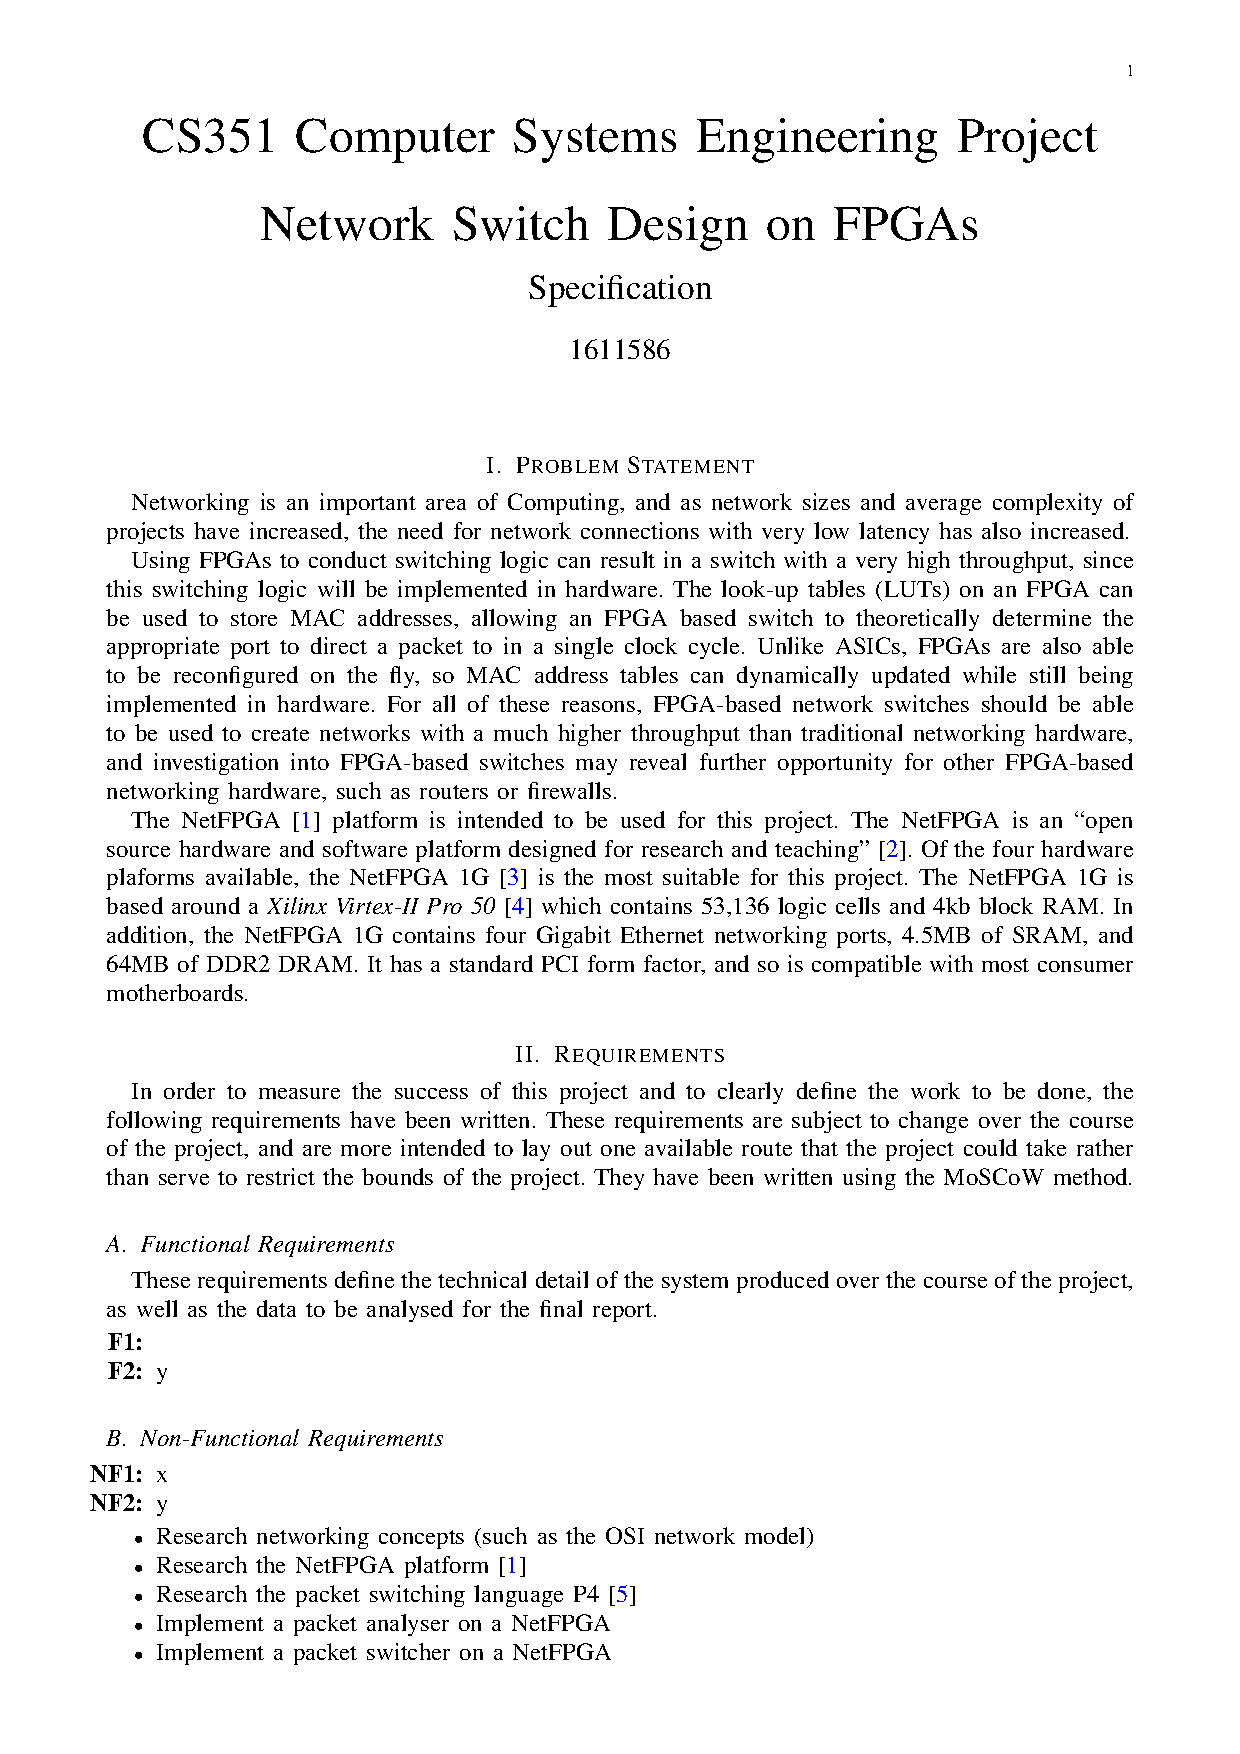
\includepdf[pages=-]{specification.pdf}
% \documentclass[12pt, a4paper, twoside, onecolumn]{article}

%% Language and font encodings
\usepackage[english]{babel}
\usepackage[utf8x]{inputenc}
\usepackage[T1]{fontenc}
\usepackage{mathptmx}

%% Sets page size and margins
\usepackage[a4paper,top=2cm,bottom=1.6cm,left=1.8cm,right=1.8cm,marginparwidth=2cm]{geometry}

%% Useful packages
\usepackage{amsmath}
\usepackage{graphicx}
\usepackage{pgfgantt}
\usepackage{url}
\usepackage{xparse}
\usepackage{listings}
\usepackage[colorlinks=true, allcolors=blue]{hyperref}
\usepackage{caption}
\usepackage{lscape}
\usepackage{enumitem}

\hypersetup{
    colorlinks = false
}

%% Section Numbering
%\setcounter{secnumdepth}{0} % no sections will be numbered
%\setcounter{secnumdepth}{1} % only sections will be numbered
%\setcounter{secnumdepth}{2} % sections and subsections will be numbered
%\setcounter{secnumdepth}{3} % sections, subsections and subsubsections will be numbered

%% TrueType font for code. use \codeword{} around sections of code in your document
\NewDocumentCommand{\codeword}{v}{
  \texttt{\textcolor{black}{#1}}
}

% You may want to use \vspace{-1cm} at times to change vertical spacing in a slightly hacky but functional way

\title{CS351 Computer Systems Engineering Project \\ \vspace{0.5cm} Network Switch Design on Field-Programmable Gate Arrays \\ \vspace{0.3cm} \Large{Specification}}
\author{1611586}

\begin{document}

\begin{titlepage}
   \begin{center}
       \vspace*{1.5cm}

      
\includegraphics[width=0.25\textwidth]{warwick_logo_old.png}

      \vspace{1.5cm}
      \textbf{Network Switch Design on FPGAs}

      \vspace{1.5cm}
      \textbf{CS351 Computer Systems Engineering Project} \\
      \vspace{0.5cm}


      \textbf{Specification}

      \vspace{4cm}

      \textbf{Benji Levine}

      \vspace{4cm}

      Superviser: Dr Suhaib Fahmy

      \vspace{0.8cm}

      Department of Computer Science\\
      University of Warwick

      \vspace{0.7cm}

      2018-19

   \end{center}
\end{titlepage}


\title{CS351 Computer Systems Engineering Project \\ \vspace{0.5cm} Network Switch Design on FPGAs \\ \vspace{0.3cm} \Large{Specification}}
\author{1611586}


\tableofcontents
\newpage

\section{Glossary}
\label{glossary}
The following acronyms are used throughout the specification:
\begin{itemize}
  \item \textbf{FPGA}: Field-Programmable Gate Array
  \item \textbf{ASIC}: Application-Specific Integrated Circuit
  \item \textbf{LUT}: Look-Up Table
\end{itemize}

\section{Problem Statement}
\label{problem_statement}
Networking is an important area of Computing, and as network sizes and average complexity of projects have increased,
the need for network connections with very low latency has also increased.

Using FPGAs to conduct switching logic can result in a switch with a very high throughput, since this switching logic will be implemented in hardware. The look-up tables (LUTs) on an FPGA can be used to store MAC addresses, allowing an FPGA based switch to theoretically determine the appropriate port to direct a packet to in a single clock cycle. Unlike ASICs, FPGAs are also able to be reconfigured on the fly, so MAC address tables can dynamically updated while still being implemented in hardware.
For all of these reasons, FPGA-based network switches should be able to be used to create networks with a much higher throughput than traditional networking hardware, and investigation into FPGA-based switches may reveal further opportunity for other FPGA-based networking hardware, such as routers or firewalls.

The NetFPGA \cite{NetFPGA} platform is intended to be used for this project. The NetFPGA is an ``open source hardware and software platform designed for research and teaching'' \cite{NetFPGA_about}. Of the four hardware plaforms available, the NetFPGA 1G \cite{NetFPGA_1G} is the most suitable for this project. The NetFPGA 1G is based around a \textit{Xilinx Virtex-II Pro 50} \cite{virtex2-pro} which contains 53,136 logic cells and 4kb block RAM. In addition, the NetFPGA 1G contains four Gigabit Ethernet networking ports, 4.5MB of SRAM, and 64MB of DDR2 DRAM. It has a standard PCI form factor, and so is compatible with most consumer motherboards.

\section{Requirements}
\label{requirements}
In order to measure the success of this project and to clearly define the work to be done, the following requirements have been written. These requirements are subject to change over the course of the project, and are more intended to lay out one available route that the project could take rather than serve to restrict the bounds of the project. They have been written using the MoSCoW method.

\subsection{Functional Requirements}
\label{functional_requirements}

These requirements define the technical detail of the system produced over the course of the project, as well as the data to be analysed for the final report.
\begin{enumerate}[label=\textbf{F\arabic*:}]
  \item The system \textbf{must} be able to analyse packets at layer 2 of the OSI network model
  \item The system \textbf{must} be able to send packets to the correct port based on MAC addresses
  \item The system \textbf{must} be able to store MAC address tables
  \item The system \textbf{must} be able to keep MAC address tables up to date
  \item The average latency of the system \textbf{must} be measured
  \item The throughput of the system \textbf{must} be measured
  \item The system \textbf{should} be able to analyse packets at layer 3 of the OSI network model
  \item The system \textbf{could} be able to analyse packets at layer 7 of the OSI network model
  \item The system \textbf{could} be able to detect basic network attacks (such as SYN Flooding \cite{rfc4987})
  \item The system \textbf{could} implement features of a basic firewall (such as packet filtering \cite{rfc2979})
\end{enumerate}

\subsection{Non-Functional Requirements}
\label{non_functional_requirements}
\begin{enumerate}[label=\textbf{NF\arabic*:}]
  \item The system \textbf{should} be scalable
  \item All code for the system \textbf{should} be well documented and maintainable
  \item The system \textbf{should} be efficient
\end{enumerate}

\section{Objectives}
\label{objectives}

\begin{itemize}
  \item Research networking concepts (such as the OSI network model)
  \item Research the NetFPGA platform \cite{NetFPGA}
  \item Research the packet switching language P4 \cite{P4}
  \item Implement a packet analyser on a NetFPGA
  \item Implement a packet switcher on a NetFPGA
  \item Test throughput and latency of switching packets using the NetFPGA packet switcher
  \item Test throughput and latency of switching packets using a conventional network switch
  \item Compare performance of NetFPGA packet switcher to conventional network switch
  \item Write up performance comparison
\end{itemize}

\section{Project Management}
\label{project_management}

\subsection{Methods}
\label{methods}
This project will use an agile methodology so that it can adapt to changes which arise during the project. Since the research and implementation stages of the project will contribute to confirming the direction the project will take, this flexibilty is important. In addition, git \cite{git} will be used to track changes in both written documents and any code developed for the project, such as any P4 or Verilog code. Repositories will be set up in git for the different areas of the project, and these repositories will be stored primarily on an online GitHub \cite{github} server and will be backed up regularly. A Gantt chart (shown in figure \ref{gantt_chart}) has been constructed to show an outline of the project timetable, and is intended to be flexible to changes arising during the course of the project.

\subsection{Timetable}
\label{timetable}

\begin{landscape}
\begin{figure}
  \begin{center}
  \begin{ganttchart}[hgrid, vgrid]{1}{32}
    \gantttitle{Term 1}{10}
    \gantttitle{Christmas}{4}
    \gantttitle{Term 2}{10}
    \gantttitle{Easter}{5}
    \gantttitle{Term 3}{3} \\
    \gantttitlelist{1,...,10}{1}
    \gantttitlelist{1,...,4}{1}
    \gantttitlelist{1,...,10}{1}
    \gantttitlelist{1,...,5}{1}
    \gantttitlelist{1,...,3}{1} \\
    % \ganttgroup{Initial Research}{2}{7} \\
    \ganttbar[name=write_spec]{Write Specification}{1}{2} \\
    \ganttmilestone[name=submit_spec]{Submit Specification}{2} \\
    \ganttbar[name=r_network]{Research Networking Concepts}{3}{3} \\
    \ganttbar[name=r_netfpga]{Research NetFPGA}{4}{4} \\
    \ganttbar[name=r_p4]{Research P4}{5}{6} \\
    \ganttbar[name=write_prog]{Write Progress Report}{7}{9} \\
    \ganttmilestone[name=submit_prog]{Submit Progress Report}{9} \\
    \ganttbar[name=implement_pa]{Implement a Packet analyser on NetFPGA}{10}{16} \\
    \ganttbar[name=implement_ps]{Implement a Packet Switcher on NetFPGA}{17}{20} \\
    \ganttbar[name=compare_speed]{Compare latency of NetFPGA switch with conventional switch}{21}{21} \\
    \ganttbar[name=prep_presentation]{Prepare Presentation}{22}{23} \\
    \ganttmilestone[name=presentation]{Presentation}{23} \\
    \ganttbar[name=write_final]{Write Final Report}{24}{31} \\
    \ganttmilestone[name=submit_final]{Submit Final Report}{31} \\
    \ganttlink{write_spec}{submit_spec}
    \ganttlink{submit_spec}{r_network}
    \ganttlink{r_network}{r_netfpga}
    \ganttlink{r_netfpga}{r_p4}
    \ganttlink{r_p4}{write_prog}
    \ganttlink{write_prog}{submit_prog}
    \ganttlink{submit_prog}{implement_pa}
    \ganttlink{implement_pa}{implement_ps}
    \ganttlink{implement_ps}{compare_speed}
    \ganttlink{compare_speed}{prep_presentation}
    \ganttlink{prep_presentation}{presentation}
    \ganttlink{presentation}{write_final}
    \ganttlink{write_final}{submit_final}
  \end{ganttchart}
  \caption{Gantt Chart of Project Timetable}
  \label{gantt_chart}
\end{center}
\end{figure}
\end{landscape}


\section{Resources}
\label{resources}
This project will use a number of different resources, including hardware, software, and languages. These are listed below.
\begin{itemize}
  \item git \cite{git}
    \begin{itemize}
      \item git will be used for version control of all code and documents
    \end{itemize}
  \item GitHub \cite{github}
    \begin{itemize}
      \item Will be used as an external server to store code and documents, as well as an interface to git
    \end{itemize}
  \item NetFPGA \cite{NetFPGA}
    \begin{itemize}
      \item Will be used as the platform on which a switch is developed
    \end{itemize}
  \item P4 \cite{P4}
    \begin{itemize}
      \item Will be used to implement packet switching on the NetFPGA
    \end{itemize}
  \item LaTeX \cite{latex}
    \begin{itemize}
      \item Will be used to write and format all documents
    \end{itemize}
  \item Atom \cite{atom}
    \begin{itemize}
      \item Will be used as an editor to write code
    \end{itemize}
\end{itemize}


\bibliographystyle{ieeetr}
\bibliography{bibliography}

\end{document}



\end{document}
